% use pdf version 1.4
\pdfoptionpdfminorversion=4

\documentclass[twoside, 12pt, a4paper, ngerman, final]{report}

% Document properties %%%%%%%%%%%%%%%%%%%%%%%%%%%%%%%%%%%%%%%%%%%%%%%%%%%%%%%%
%%%%%%%%%%%%%%%%%%%%%%%%%%%%%%%%%%%%%%%%%%%%%%%%%%%%%%%%%%%%%%%%%%%%%%%%%%%%%%

\pdfinfo{
	/Author   (Anselm Busse)
	/Title    (Analyse der Diversifikation im Bankensektor als Ursache systemischer Risiken)
	/Subject  (Bachelorarbeit)
	/Keywords (Systemische Risiken, Banken, Diversifikation)
}

% Included packages %%%%%%%%%%%%%%%%%%%%%%%%%%%%%%%%%%%%%%%%%%%%%%%%%%%%%%%%%%%%
%%%%%%%%%%%%%%%%%%%%%%%%%%%%%%%%%%%%%%%%%%%%%%%%%%%%%%%%%%%%%%%%%%%%%%%%%%%%%%%%

\usepackage{morewrites}					% we will need more than 16 write handles
\usepackage[utf8]{inputenc}				% use UTF-8 input encoding
\usepackage{lmodern}
\usepackage[T1]{fontenc}				% western font encoding, improve hyphenation
\usepackage{textcomp}
\usepackage{tipa}						% Text-mode Accents (e.g. \textpolhook{a})
\usepackage[main=ngerman, english]{babel}% set main language
\usepackage{ifdraft}					% enable check for draft option
\usepackage{mathtools}					% display equations
\usepackage{amssymb}					% math symbols
\usepackage{wasysym}					% additional symbols
\usepackage{amsfonts}
\usepackage{xspace}						% control whitspaces after macros
\usepackage[hang,bottom]{footmisc}		% footnote modifications
\usepackage{geometry}					% general page layout
\usepackage{fancyhdr}
\usepackage{sectsty}
\usepackage{graphicx}
\usepackage{scrextend}					% reference footnotes
\usepackage[hang,bf,					% hang caption, bf
            tableposition=top,			% table caption is always above table
            margin=20pt]{caption}		% indent caption
\usepackage[listformat=simple,			% subfigure caption
            list=true]{subcaption}		% list subfigures in table of figures
\usepackage[titles,subfigure]{tocloft}	% define new 'List of...' and TOC layout
\usepackage{floatrow}					% enables caption above listing, load before minted
\usepackage{framed}
\usepackage[autostyle,
            english=american,
            german=guillemets]{csquotes}
\usepackage{savesym}
\savesymbol{checkmark}
\usepackage{mdwlist}
\usepackage[normalem]{ulem}				% underlinging (e.g. \sout and \uwave)
\usepackage{extramarks}
\usepackage{enumitem}					% change the itemize front character
\usepackage{float}
\usepackage[]{acronym}					% handle acronyms
\usepackage{array}						% improved tabular environment
\usepackage{pgfplots, pgfplotstable}
\usepackage{xcolor}				        % enable eg color names (load before tikz!!!)
\usepackage{tikz}			            % lets draw some stuff like a boss
\usepackage{chngcntr}					% custom counteres used for e.g. time and date calculation
\usepackage{xspace}						% enable conditional withespace for e.g. a.s.o.
\usepackage[super]{nth}					% superscript st, nd, rd, th
\usepackage{wrapfig}					% wrap text around figures
\usepackage[figuresright]{rotating}		% rotate figures
\usepackage{textgreek}					% greek letter in text mode \textalpha etc.
\usepackage{relsize}
\usepackage[chapter]{algorithm}
\usepackage[]{algpseudocode}
\usepackage{multicol}					% introduce multicolumn environment
\usepackage{multirow}
\usepackage{tabularx}
\usepackage{colortbl}
\usepackage{tcolorbox}					% colored table boxes
\usepackage{dirtree}					% directory listings
\usepackage{booktabs}
\usepackage{xtab}						% tables spanning multiple pages
\usepackage{threeparttable}				% table with footnotes
\usepackage{environ}
\usepackage[nodisplayskipstretch]{setspace}					% allow to set line spacing
\usepackage{afterpage}					% put text/figure after a certain page
\usepackage[locale=DE,
            detect-weight=true,
            detect-family=true]{siunitx}			% numbers and units
\usepackage{xpatch}						% allow some bib patching
\usepackage{fnpct}						% improve footnote reference placing
\usepackage[nosuper]{glossaries}
\usepackage{physics}
\usepackage{ziffer}						% german number seperators

% Improve overall appearance with microtype package %%%%%%%%%%%%%%%%%%%%%%%%%%%%
% read http://www.khirevich.com/latex/microtype/ for further information %%%%%%%
%%%%%%%%%%%%%%%%%%%%%%%%%%%%%%%%%%%%%%%%%%%%%%%%%%%%%%%%%%%%%%%%%%%%%%%%%%%%%%%%
\usepackage[activate={true,nocompatibility},	% activate protrusion and expansion
            final,
            tracking=true,
            kerning=true,
            spacing=true,
            factor=1100,						% add 10% to the protrusion amount (default is 1000)
            stretch=10,
            shrink=10]{microtype}

% PDF setup with links %%%%%%%%%%%%%%%%%%%%%%%%%%%%%%%%%%%%%%%%%%%%%%%%%%%%%%%%%
%%%%%%%%%%%%%%%%%%%%%%%%%%%%%%%%%%%%%%%%%%%%%%%%%%%%%%%%%%%%%%%%%%%%%%%%%%%%%%%%

\usepackage[a-1b]{pdfx}
\hypersetup{final,            %links are only inserted in final mode
            %pdfpagemode={UseOutlines},
            bookmarksopen=false,bookmarksopenlevel=0,
            bookmarksnumbered=true,
            hypertexnames=false,
            pdfstartview={FitV},
            colorlinks=false,linkcolor={black},citecolor={black},urlcolor={black},
            linktoc=all,
            breaklinks=true,
            %pagebackref=true,
            plainpages=false,
            pageanchor=true,
            %backref=page
            }
\PassOptionsToPackage{dvipsnames}{xcolor}

\usepackage[capitalise]{cleveref}		% more sophisticated references 
										%(load after hyperref!)

% Packages specific for draft and debugging %%%%%%%%%%%%%%%%%%%%%%%%%%%%%%%%%%%%
%%%%%%%%%%%%%%%%%%%%%%%%%%%%%%%%%%%%%%%%%%%%%%%%%%%%%%%%%%%%%%%%%%%%%%%%%%%%%%%%
\usepackage{showlabels}					% prints LaTex lables in draft mode

% Reduce label size of showlabels package
\renewcommand{\showlabelfont}{\scriptsize}

% Bibliography setup %%%%%%%%%%%%%%%%%%%%%%%%%%%%%%%%%%%%%%%%%%%%%%%%%%%%%%%%%%%
%%%%%%%%%%%%%%%%%%%%%%%%%%%%%%%%%%%%%%%%%%%%%%%%%%%%%%%%%%%%%%%%%%%%%%%%%%%%%%%%
\usepackage[backend=biber,
            bibencoding = utf8,
            natbib = true,
            style = authoryear-comp,
            giveninits=true,
            uniquename=init,
            maxnames = 12,
            minnames = 1,
            maxcitenames=2,
            backref = false,
            backrefstyle = two,
            defernumbers = true,
            isbn=true,
            doi=true,
            dashed=false,
            %backref=true,			% enable to show refering pages in entry
            ]{biblatex}

% Bibliography files
\addbibresource{thesis-main.bib}

\DeclareBibliographyAlias{software}{online}

\DeclareDelimFormat[cbx@textcite]{nameyeardelim}{\addspace}

\DeclareFieldFormat[techreport,report,unpublished]{title}{\mkbibquote{#1}}

\DeclareFieldFormat{edition}{\ifinteger{#1}%
							 {\mkbibordedition{#1}\addthinspace{}ed.}%
							 {#1\isdot}
							}

% redefine strings in Bibliography
\DefineBibliographyStrings{english}{%
	urlseen = {Retrieved},  
	sequens = {f\adddot},			% use f. instead of sq.
	sequentes = {ff\adddot},		% use ff. instead of sqq.
}

\renewcommand*{\sqspace}{}			% no space at \psq and \psqq

\assignrefcontextkeyws[labelprefix=S]{software}

% only print isbn or issn if doi is not present
\DeclareSourcemap{
	\maps[datatype=bibtex]{
		\map{
			\step[fieldsource=doi,final]
			\step[fieldset=isbn,null]
		}
		\map{
			\step[fieldsource=doi,final]
			\step[fieldset=issn,null]
		}
	}
}

\DeclareSortingScheme{ymdnt}{
	\sort{
		\field{presort}
	}
	\sort[final]{
		\field{sortkey}
	}
	\sort[direction=descending]{
		\field[strside=left,strwidth=4]{sortyear}
		\field[strside=left,strwidth=4]{year}
		\literal{9999}
	}
	\sort[direction=descending]{
		\field{month}
		\literal{9999}
	}
	\sort{
		\field{sortname}
		\field{author}
		\field{editor}
		\field{translator}
		\field{sorttitle}
		\field{title}
	}
	\sort{
		\field{sorttitle}
		\field{title}
	}
}

\renewcommand\namelabeldelim{\addnbspace}
%\renewcommand\multicitedelim{\addcomma\addnbspace}
\defcounter{abbrvpenalty}{10000}

% Make sure that not overful hboxes are created through URLs
\setcounter{biburllcpenalty}{7000}
\setcounter{biburlucpenalty}{8000}

% Page setup via geometry package %%%%%%%%%%%%%%%%%%%%%%%%%%%%%%%%%%%%%%%%%%%%
%%%%%%%%%%%%%%%%%%%%%%%%%%%%%%%%%%%%%%%%%%%%%%%%%%%%%%%%%%%%%%%%%%%%%%%%%%%%%%

\geometry{a4paper,centering}
\geometry{hmargin={3cm, 3cm},vmargin={3cm,3cm}}


%%%%%%%%%%%%%%%%%%%%%%%%%%%%%%%%%%%%%%%%%%%%%%%%%%%%%%%%%%%%%%%%%%%%%%%%%%%%%%%%

% Calculation of current time based on counter \time (minutes since midnight)
% Usage: \now
\newcount\myhours
\newcount\myminutes
\myhours   = \time \divide \myhours by 60
\myminutes = \time \multiply \myhours by 60 \advance \myminutes by -\myhours
             \divide \myhours by 60
\def\now{\ifnum\myhours<10{}0\fi\number\myhours:\ifnum\myminutes<10{}0\fi\number\myminutes}

% Adds a <line> to the Table of Contents (TOC)
% Usage: \addtotoc{<line>}
\newcommand{\addtotoc}[1]{
  \ifnum0=\csname c@section\endcsname
    \def\myLevel{section}
    \def\myEntry{#1}
  \else
    \ifnum0=\csname c@subsection\endcsname
      \def\myLevel{section}
      \def\myEntry{\protect\numberline{}{#1}}
    \else
      \def\myLevel{subsection}
      \def\myEntry{\protect\numberline{}{#1}}
    \fi
  \fi
  \addcontentsline{toc}{\myLevel}{\myEntry}
}

% Defines a TODO <aspect> that is only visible in draft mode
% Usage: \TODO{<aspect>} simply adds a blue todo to the text
%        \TODO[<description>]{<aspect>} also adds <description> to the TOC
\ifdraft{
	\newcommand{\TODO}[2][@]{
		{\textcolor{blue}{[TODO: #2]}}
		\ifx#1@
		\else
      		\addtotoc{\textcolor{blue}{TODO: #1}}
    	\fi
  	}
	\newcommand{\QUEST}[2][@]{
		{\textcolor{red}{[Question: #2]}}
		\ifx#1@
		\else
      		\addtotoc{\textcolor{red}{Question: #1}}
    	\fi
  	}
}{
	\newcommand{\TODO}[2][@]{}
	\newcommand{\QUEST}[2][@]{}
}

\newcommand{\TR}{\ref{TODO}\TODO{Missing Reference}\@\xspace\PackageWarning{TODO}{Missing Reference}}
\newcommand{\TC}{\cite{TODO}\TODO{Missing Citation}\@\xspace\PackageWarning{TODO}{Missing Citation}}

% Underlines <passage>s that should be checked later (visible in draft mode)
% Usage \CHECK{<passage>}
\ifdraft{
  \newcommand{\CHECK}[1]{\uwave{#1}}
}{
  \newcommand{\CHECK}[1]{#1}
}

% Alternative to commenting out <paragraphs>
% Usage: \FORGET{<paragraphs>}
\ifdraft{
  \newcommand{\FORGET}[1]{\sout{#1}}
}{
  \newcommand{\FORGET}[1]{}
}

\newcommand*{\eg}{e.g.\@\xspace}
\newcommand*{\ie}{i.e.\@\xspace}
\newcommand*{\cf}{cf.\xspace}
\newcommand*{\etal}{et\ al.\@\xspace}

\newcommand*{\zb}{z.B.\@\xspace}
\newcommand*{\vgl}{vgl.\@\xspace}
\newcommand*{\bzw}{bzw.\@\xspace}
\newcommand*{\ua}{u.a.\@\xspace}

\newcommand{\rpm}{\sbox0{$1$}\sbox2{$\scriptstyle\pm$}
  \raise\dimexpr(\ht0-\ht2)/2\relax\box2 }

\renewcommand{\l}[1]{l\adddot~#1}
\renewcommand{\ll}[1]{ll\adddot~#1}

\newcommand*{\elide}{\textup{[\,\dots]}\@\xspace}

\newcommand{\breakL}[1]{\begin{tabular}{l}#1\end{tabular}}
\newcommand{\breakC}[1]{\begin{tabular}{c}#1\end{tabular}}
\newcommand{\breakR}[1]{\begin{tabular}{r}#1\end{tabular}}

\DeclareMathOperator*{\argmin}{arg\,min}

\newcommand{\Lim}[1]{\raisebox{0.5ex}{\scalebox{0.8}{$\displaystyle \lim_{#1}\;$}}}

% Just load the \drsh character from mathabx as it is as a whole incompatible with ams
\DeclareFontFamily{U}{mathb}{\hyphenchar\font45}
\DeclareFontShape{U}{mathb}{m}{n}{
      <5> <6> <7> <8> <9> <10> gen * mathb
      <10.95> mathb10 <12> <14.4> <17.28> <20.74> <24.88> mathb12
      }{}
\DeclareSymbolFont{mathb}{U}{mathb}{m}{n}
\DeclareMathSymbol{\drsh}                  {3}{mathb}{"EB}

% Fonts %%%%%%%%%%%%%%%%%%%%%%%%%%%%%%%%%%%%%%%%%%%%%%%%%%%%%%%%%%%%%%%%%%%%%%%%
%%%%%%%%%%%%%%%%%%%%%%%%%%%%%%%%%%%%%%%%%%%%%%%%%%%%%%%%%%%%%%%%%%%%%%%%%%%%%%%%

% Set fonts for headlines, tables, and listings
\allsectionsfont{\bfseries}
\sisetup{math-micro=\text{\textmugreek},
		 text-micro=\textmugreek,
		 exponent-product=\cdot,
		 output-product=\cdot}

% Page Layout %%%%%%%%%%%%%%%%%%%%%%%%%%%%%%%%%%%%%%%%%%%%%%%%%%%%%%%%%%%%%%%%
%%%%%%%%%%%%%%%%%%%%%%%%%%%%%%%%%%%%%%%%%%%%%%%%%%%%%%%%%%%%%%%%%%%%%%%%%%%%%%
% Standard header and footer
\setlength{\headheight}{14.6pt}
\renewcommand{\headrulewidth}{0pt}

\fancypagestyle{frontmatter}{
	\fancyhf{}
	\fancyheadoffset[OR,EL]{2.4cm}
	\fancyhead[OR]{\textsc{\nouppercase{\leftmark}}\quad\smash{\rule[-.2ex]{1pt}{4cm}}\quad\makebox[\widthof{0000000}][l]{\thepage}}
	\fancyhead[EL]{\makebox[\widthof{0000000}][r]{\thepage}\quad\smash{\rule[-.2ex]{1pt}{4cm}}\quad\textsc{\nouppercase{\leftmark}}}
}


\fancypagestyle{mainmatter}{
	\fancyhf{}
	\fancyheadoffset[OR,EL]{2.4cm}
	\fancyhead[OR]{\textsc{\nouppercase{\rightmark}}\quad\smash{\rule[-.2ex]{1pt}{4cm}}\quad\makebox[\widthof{0000000}][l]{\thepage}}
	\fancyhead[EL]{\makebox[\widthof{0000000}][r]{\thepage}\quad\smash{\rule[-.2ex]{1pt}{4cm}}\quad\textsc{\nouppercase{\leftmark}}}
}

\fancypagestyle{backmatter}{
	\fancyhf{}
	\fancyheadoffset[OR,EL]{2.4cm}
	\fancyhead[OR]{\textsc{\nouppercase{\rightmark}}\quad\smash{\rule[-.2ex]{1pt}{4cm}}\quad\makebox[\widthof{0000000}][l]{\thepage}}
	\fancyhead[EL]{\makebox[\widthof{0000000}][r]{\thepage}\quad\smash{\rule[-.2ex]{1pt}{4cm}}\quad\textsc{\nouppercase{\leftmark}}}
}

% header and footer on other pages
\fancypagestyle{plain}{
	\fancyhead{}
	\fancyfoot[CE,CO]{\sffamily\thepage}
	\ifdraft{
		\fancyfoot[C]{\today, \now}
		\fancyfoot[R]{\sffamily\thepage}
	}{
		\fancyfoot[C]{}
		\fancyfoot[R]{\thepage}
	}
}

% Paragraphs and footnotes
\setlength\parskip{\medskipamount}
\setlength\parindent{0pt}
\setlength\footnotemargin{0.8em}
\setlength{\headheight}{15pt} 

% Chapter layout

\usepackage{titlesec}
\titleformat{\chapter}[display]
	{\normalfont\Large\raggedleft}% format
	{\raggedleft\MakeUppercase{\chaptertitlename~\thechapter}}  % label
	{0ex} % sep
	{\Huge\bfseries} % before-code
	[\vspace{-3ex}%
	 \rule{\textwidth}{0.3pt}
	] % after-code
\titleformat{name=\chapter,numberless}[display]
	{\normalfont\Large\raggedleft}% format
	{}  % label
	{-3ex} % sep
	{\Huge\bfseries} % before-code
	[\vspace{-2ex}%
	 \rule{\textwidth}{0.3pt}
	] % after-code

\titleformat*{\section}{\Large\bfseries}
\titleformat*{\subsection}{\large\bfseries}
\titleformat*{\subsubsection}{\large\bfseries}
\titleformat*{\paragraph}{\large\bfseries}
\titleformat*{\subparagraph}{\large\bfseries}

\titlespacing*{\chapter}{0pt}{-3em}{0pt}
\titlespacing{\section}{0pt}{5pt}{5pt}
\titlespacing{\subsection}{0pt}{5pt}{5pt}
\titlespacing{\subsubsection}{0pt}{5pt}{5pt}
\titlespacing{\paragraph}{0pt}{5pt}{5pt}

% The subfigure option of the tocloft package needs the 'lofdepth' & 'lotdepth'
% counter. Normally its define by the subfigure or subfig package, but as we use
% subcaption we have to define it on our own
\newcounter{lofdepth}
\setcounter{lofdepth}{2}
\newcounter{lotdepth}
\setcounter{lotdepth}{2}

% Document specific commands and abbreviations %%%%%%%%%%%%%%%%%%%%%%%%%%%%%%%%%
%%%%%%%%%%%%%%%%%%%%%%%%%%%%%%%%%%%%%%%%%%%%%%%%%%%%%%%%%%%%%%%%%%%%%%%%%%%%%%%%

\floatsetup[listing]{style=plaintop}
\floatstyle{plaintop}
\restylefloat{table}

\makeatletter 
\def\mod@estimate@lineht{% 
  \ST@lineht=\arraystretch \baslineskp 
  %\global\advance\ST@lineht by 1\p@ 
  \ST@stretchht\ST@lineht\advance\ST@stretchht-\baslineskp 
  \ifdim\ST@stretchht<\z@\ST@stretchht\z@\fi 
  \ST@trace\tw@{Average line height: \the\ST@lineht}% 
  \ST@trace\tw@{Stretched line height: \the\ST@stretchht}% 
} 
\newenvironment{strictsupertabular} 
  {\let\estimate@lineht\mod@estimate@lineht\supertabular} 
  {\endsupertabular} 
\makeatother

% Change the itemize symbols

\def\labelitemi{\normalfont \bfseries \textendash}
\def\labelitemii{\textasteriskcentered}

% correct spacing

\BeforeBeginEnvironment{align}{\begin{singlespace}\vspace*{-\baselineskip}}
\AfterEndEnvironment{align}{\end{singlespace}\noindent\ignorespaces}
\BeforeBeginEnvironment{align*}{\begin{singlespace}\vspace*{-\baselineskip}}
\AfterEndEnvironment{align*}{\end{singlespace}\noindent\ignorespaces}
\BeforeBeginEnvironment{gather}{\begin{singlespace}\vspace*{-\baselineskip}}
\AfterEndEnvironment{gather}{\end{singlespace}\noindent\ignorespaces}
\BeforeBeginEnvironment{figure}{\begin{singlespace}\vspace*{-\baselineskip}}
\AfterEndEnvironment{figure}{\end{singlespace}\noindent\ignorespaces}

\AdaptNoteOpt\footcite\multfootcite
\setfnpct{after-punct-space=-0.12em}

\setstretch{1.5}

% don't footnote numbers with 1 every chapter %%%%%%%%%%%%%%%%%%%%%%%%%%%%%%%%%%
%%%%%%%%%%%%%%%%%%%%%%%%%%%%%%%%%%%%%%%%%%%%%%%%%%%%%%%%%%%%%%%%%%%%%%%%%%%%%%%%
\counterwithout{footnote}{chapter}

% TikZ setup %%%%%%%%%%%%%%%%%%%%%%%%%%%%%%%%%%%%%%%%%%%%%%%%%%%%%%%%%%%%%%%%%%%
%%%%%%%%%%%%%%%%%%%%%%%%%%%%%%%%%%%%%%%%%%%%%%%%%%%%%%%%%%%%%%%%%%%%%%%%%%%%%%%%

\usetikzlibrary{arrows,arrows.meta,bending}

\tikzset{
    %Define standard arrow tip
    >=stealth',
}

\definecolor{normal}{RGB}{203,255,181}		
\definecolor{individual}{RGB}{253,249,192}	
\definecolor{system}{RGB}{255,130,130}
\definecolor{error}{RGB}{173,220,236}

\definecolor{graph1}{rgb}{0.106,0.620,0.467}
\definecolor{graph2}{rgb}{0.851,0.373,0.008}
\definecolor{graph3}{rgb}{0.459,0.439,0.702}

\newcommand{\includetikz}[1]{\input{#1.tikz}}

% Use a recent version for tikz and pgf plotting
\pgfplotsset{compat=1.14}

%!TEX root = bachelor.tex

\makeglossaries
\renewcommand*{\glossaryname}{Symbolverzeichnis}
\deftranslation{Glossary}{Symbolverzeichnis}
\renewcommand*{\glspostdescription}{}

\setlength{\glslistdottedwidth}{.14\linewidth}

\newglossaryentry{symb:pis}{
name=$\pi^S$,
description={Wahrscheinlichkeit einer systemischen Krise.},
sort=symbolt
}

\newglossaryentry{symb:pi1}{
name=$\pi^I_i$,
description={Wahrscheinlichkeit einer individuellen Krise der Bank $i$.},
sort=symbolt
}

\newglossaryentry{symb:pii}{
name=$\pi_i$,
description={Wahrscheinlichkeit einer Krise der Bank $i$.},
sort=symbolt
}

\newglossaryentry{symb:d}{
name=$d$,
description={Anteil der Einlagen am Gesamtkapital einer Bank.},
sort=symbolt
}

\newglossaryentry{symb:x}{
name=$x$,
description={Tatsächliche Realisierung des Werts der Anlage $X$.},
sort=symbolt
}

\newglossaryentry{symb:y}{
name=$y$,
description={Tatsächliche Realisierung des Werts der Anlage $Y$.},
sort=symbolt
}

\newglossaryentry{symb:c}{
name=$c$,
description={Verlust beim Transfer einer Anlage zwischen Banken.},
sort=symbolt
}

\newglossaryentry{symb:q}{
name=$q$,
description={Verlustfaktor bei vorzeitiger Liquidierung einer Anlage.},
sort=symbolt
}

\newglossaryentry{symb:vi}{
name=$v_i$,
description={Wert der Bank $i$.},
sort=symbolt
}

\newglossaryentry{symb:phi}{
name=$\phi$,
description={Eine Wahrscheinlichkeitsdichtefunktion für eine beliebige Verteilung mit kompakten Intervall.},
sort=symbolt
}

\newglossaryentry{symb:s}{
name=$s$,
description={Höchstmögliche Realisierung des Werts einer Anlage.},
sort=symbolt
}

\newglossaryentry{symb:ri}{
name=$r_i$,
description={Diversifizierungsgrad der Bank $i$.},
sort=symbolt
}

\newglossaryentry{symb:roptall}{
name=$r^\ast$,
description={Volkswirtschaftlich optimaler Diversifizierungsgrad der Banken.},
sort=symbolt
}

\newglossaryentry{symb:roptone}{
name=$r^E$,
description={Individuell optimaler Diversifizierungsgrad einer Bank.},
sort=symbolt
}


\begin{document}

% Preface %%%%%%%%%%%%%%%%%%%%%%%%%%%%%%%%%%%%%%%%%%%%%%%%%%%%%%%%%%%%%%%%%%%%
%%%%%%%%%%%%%%%%%%%%%%%%%%%%%%%%%%%%%%%%%%%%%%%%%%%%%%%%%%%%%%%%%%%%%%%%%%%%%%

\renewcommand{\thepage}{\roman{page}}

\microtypesetup{protrusion=true}

%!TEX root = bachelor.tex

\newgeometry{hmargin={2cm, 2cm},vmargin={2cm,2cm}}
\pdfbookmark{Titelblatt}{Titelblatt}

\begin{titlepage}
	\singlespacing{} \sffamily

	\begin{figure} \sffamily
		\begin{flushright}
			\begin{tabular}[m]{r}
				Technische Universität Berlin           \\
				Fakultät Wirtschaft und Management      \\
				Institut für Betriebswirtschaftslehre   \\
				Fachgebiet Finanzierung und Investition \\
			\end{tabular}%
			\begin{tabular}[m]{c}
				
\includegraphics[height=65pt]{figures/tu-logo}
			\end{tabular}
		\end{flushright}
	\end{figure}

	\begin{center}
		\rule{0pt}{0pt}
		\vfill
		\vfill

		\begin{Huge}
			\bf\sffamily
			Analyse der Diversifikation\\[0.5ex]
			im Bankensektor\\[0.5ex]
			als Ursache systemischer Risiken\\[0.5ex]
		\end{Huge}

		\vfill
		\vfill

		\begin{LARGE}
			\bf\sffamily
			Bachelorarbeit
		\end{LARGE} \\
		\vspace{.5cm}
		vorgelegt von \\
		\vspace{.5cm}
		\begin{Large}
			\bf\sffamily
			Anselm Busse
		\end{Large} \\ \vspace{.25cm}

		Matrikelnummer 306686 \\

		\vfill
		\vfill
		\vfill
		\vfill
		\vfill


		\begin{tabular}{rl}
			Referent:    & Prof. Dr. Hans Hirth \\
			Korreferent: & Dr. Martin Walther   \\
		\end{tabular}

		\vfill

		Berlin, den 9.~Oktober 2017

	\end{center}
\end{titlepage}

\restoregeometry{}
    \cleardoublepage{}
%!TEX root = bachelor.tex

\vspace*{\fill}

Ich erkläre hiermit an Eides Statt, dass ich die vorliegende Bachelorarbeit selbstständig und ohne unerlaubte Hilfe angefertigt, andere als die angegebenen Quellen und Hilfsmittel nicht benutzt und die benutzten Quellen wörtlich oder inhaltlich entnommene Stellen als solche kenntlich gemacht habe. \newline \newline
Berlin, den 9.~Oktober 2017 \newline \newline
\hbox{} \dotfill \hspace{7.5cm} \hbox{} \newline
\hbox{} \begin{small}
Unterschrift
\end{small}
  \cleardoublepage{}
%!TEX root = bachelor.tex

\begingroup
\singlespacing{}
\chapter*{Zusammenfassung}
\endgroup

Systemische Krisen stellen eine substantielle Gefahr für jede Volkswirtschaft dar. Aus diesem Grund ist die Untersuchung der Risiken, die zu solch einer Krise führen, unabdingbar. Auslöser einer systemischen Krise kann die gleichzeitige Insolvenz aller oder mehrerer Banken sein. Obwohl Diversifizierung das individuelle Risiko einer Bank bezüglich einer Insolvenz verringern kann, kann diese Diversifizierung das Risiko einer systemischen Krise vergrößern. Diese Problematik wird in der Veröffentlichung von \emph{Wolf Wagner} mit dem Titel \mkbibquote{Diversification at Financial Institutions and Systemic Crises} detailliert diskutiert.

Die vorliegende Arbeit stellt die Erkenntnisse von Wagner ausführlich dar. Es wird dabei anhand eines 2-Banken-Modells erläutert, wie und in welchem Ausmaß Diversifikation zwar das individuelle Risiko einer Bank verringern kann, gleichzeitig jedoch das Risiko einer systemischen Krise steigert. Wagner kommt zu dem Schluss, dass eine vollständige Diversifikation aus diesem Grund nicht optimal sein kann und quantifiziert den optimalen Diversifizierungsgrad für konkrete Beispiele. Er kommt dabei zu der Erkenntnis, dass ohne eine Regulierung im Bankensektor ein zu hoher Diversifizierungsgrad präferiert wird.

Wagners Ausarbeitung wird im Rahmen dieser Arbeit in drei Aspekten kritisch hinterfragt. Zunächst werden Modellparameter untersucht, die bei Wagner keine Rücksicht fanden. Dadurch wird seine Modellanalyse komplettiert. Als zweiter Aspekt der kritischen Untersuchung wird gezeigt, dass Wagners Modell auch auf komplexere Wahrscheinlichkeitsverteilungen angewandt werden kann. Dabei werden insbesondere etwaige Probleme diskutiert, die bei der Nutzung von abschnittsweise definierten Verteilungsfunktionen entstehen. Schlussendlich findet im Rahmen dieser Arbeit eine numerische Analyse eines Bankenmarktes statt. Durch die Analyse werden Wagners Aussagen und Ergebnisse weiter untermauert.

\cleardoublepage
\begingroup
\singlespacing{}
\chapter*{Abstract}
\endgroup

\begin{otherlanguage*}{english}

Systemic crises are a great threat to every economy. Hence, it is inevitable to analyse the risks that lead to such a crisis. If several or all banks go bankrupt simultaneously, a systemic crisis might emerge. Even though diversification may minimize the risk of going bankrupt for single banks, it can also increase the chance of a systemic crisis. \emph{Wolf Wagner} discusses this problem in detail in his paper \mkbibquote{Diversification at Financial Institutions and Systemic Crises}. 

This thesis aims at presenting Wagner’s findings elaborately. Using a two financial institutions model, I will explain how and to what extent diversification is able to decrease the individual risk of a bank, yet at the same time increases the risk of a systemic crisis. Wagner concludes that a total diversification is not the best solution for this reason and furthermore quantifies the optimum grade of diversification for concrete examples.

Wagner’s work will be analysed critically with regard to three aspects. First, I will analyse the parameters that Wagner has not considered, hence completing the analysis of his model. Second, the critical examination will show that Wagner’s model is also applicable to probability distributions that are more complex. The discussion will focus especially on problems that emerge from the use of sectionally defined functions describing probability distributions. Third and last, the financial market will be examined numerically. This examination will confirm Wagner’s conclusions and results. 

\end{otherlanguage*}
     \cleardoublepage{}

% Table of contents, list of figures, etc. %%%%%%%%%%%%%%%%%%%%%%%%%%%%%%%%%%%
%%%%%%%%%%%%%%%%%%%%%%%%%%%%%%%%%%%%%%%%%%%%%%%%%%%%%%%%%%%%%%%%%%%%%%%%%%%%%%

\microtypesetup{protrusion=false}

\begingroup \singlespacing{}
	\tableofcontents \cleardoublepage{}

	\phantomsection
	\addcontentsline{toc}{chapter}{\listfigurename}
	\listoffigures
	\vspace{2.5cm}
	\begingroup
		\let\clearpage\relax
		\phantomsection
		\addcontentsline{toc}{chapter}{\listtablename}
		\listoftables
	\endgroup \cleardoublepage{}
	
	\printglossary[title={Symbolverzeichnis}, style=listdotted]
	\glsaddall{}
	\addcontentsline{toc}{chapter}{Symbolverzeichnis} \cleardoublepage{}
\endgroup

% Content %%%%%%%%%%%%%%%%%%%%%%%%%%%%%%%%%%%%%%%%%%%%%%%%%%%%%%%%%%%%%%%%%%%%
%%%%%%%%%%%%%%%%%%%%%%%%%%%%%%%%%%%%%%%%%%%%%%%%%%%%%%%%%%%%%%%%%%%%%%%%%%%%%%
\setcounter{page}{1}
\renewcommand{\thepage}{\arabic{page}}
\pagestyle{mainmatter}
\renewcommand{\chaptermark}[1]{\markboth{\thechapter\ #1}{\thechapter\ #1}}
\renewcommand{\sectionmark}[1]{\markright{\thesection\ #1}}

\microtypesetup{protrusion=true}

%!TEX root = bachelor.tex

\chapter{Einleitung}%
\label{chap:intro}

Spätestens seit der Finanzkrise ab dem Jahr 2007 sind die Möglichkeit und Folgen einer systemischen Krise in das Zentrum der Aufmerksamkeit von Öffentlichkeit und Forschung getreten. Eine systemische Krise ist eine grundlegenden Gefahr für jede Volkswirtschaft und hat dramatische Folgen, die in einer signifikanten Anzahl von Firmeninsolvenzen und massiver Verringerung des Wohlstandes in der betroffenen Volkswirtschaft führen kann. Ein Beispiel für die Konsequenzen einer solchen Krise konnten und können bis heute in Griechenland beobachtet werden (\vgl{}~\cite{Papadimitriou-2013}).

Eine zentrale Ursache für eine systemische Krise kann die gleichzeitige Insolvenz mehrere Banken sein, die zum Kollaps des gesamten Bankensektors führt, was wiederum die gesamte Geschäftstätigkeit innerhalb einer Volkswirtschaft massiv einschränkt. Somit kann dieses Szenario unstrittig als ein systemisches Risiko eingestuft werden. Als ein Mittel zur Verringerung des Risikos wird im Allgemeinen Diversifikation gesehen. Jedoch bezieht sich die Verringerung des Risikos meist nur auf das individuelle Risiko einer Bank und nicht auf das Risiko bezüglich einer systemischen Krise. Dieser Aspekt wird \ua{} von \textcite{Wagner-2010} genauer untersucht. In seiner Arbeit präsentiert \citeauthor{Wagner-2010} das Model eines Bankensektors bestehend aus zwei Banken. Er zeigt, dass durch die Diversifikation zwar das individuelle Risiko einer Bank insolvent zu werden, durch die Diversifikation sinkt, gleichzeitig aber das Risiko einer systemischen Krise steigt. Er zeigt ferner, dass ohne Regulierung die Banken in seinem Modell zu einer Überdiversifizierung neigen.

\Citeauthor{Wagner-2010} steht dabei mit seiner Feststellung, dass Diversifikation und insbesondere vollständige Diversifikation nicht zwangsläufig wünschenswert ist, nicht alleine. \Textcite{Goldstein-2004} \zb{} untersuchen die Effekte von Ansteckungen und selbsterfüllende Prophezeiungen bezüglich Krisen zwischen verschiedenen Märkten. Auch sie kommen zu dem Schluss, dass eine vollständige Diversifizierung nicht immer von Vorteil ist und das Risiko einer umfangreichen Krise erhöhen kann. Zu einem ähnlichen Schluss kommen \textcite{Danielsson-2003}. Sie untersuchen in ihrer Arbeit den Einfluss von Handelsregulierungen bezüglich Finanzmarktderivaten und wenden Ihre Erkenntnisse auf die Krisen am Schwarzen Montag 1987 und die Krise im russischen Finanzmarkt 1998 an. Neben der Erkenntnis, dass eine zwanghafte Diversifikation volkswirtschaftlich nicht optimal ist, stellen sie weiter fest, dass allgemeine Regulierungen, die für alle Marktteilnehmer und insbesondere Banken gleich sind, ebenfalls als suboptimal angesehen werden können. \Textcite{Stiglitz-2010a,Stiglitz-2010b} stellt ebenfalls fest, dass eine vollständige Diversifikation nicht wünschenswert ist. Er führt Problematiken jedoch primär auf Ansteckungen zwischen den Banken \bzw{} Märkten zurück. \Textcite{Ibragimov-2011} führen schlussendlich die Arbeit von \citeauthor{Wagner-2010} fort und vervollständigen diese insbesondere in Bezug auf alternative Risikowahrscheinlichkeiten \bzw{} Wahrscheinlichkeitsverteilungen. 

Diversifizierung kann jedoch auch aus anderen Aspekten zu systemischen Krisen führen. \Textcite{Battiston-2012} und \textcite{Teteryatnikova-2014} \zb{} untersuchen Bankennetzwerke, wobei letztere von beiden Arbeiten davon ausgeht, dass einige wenige Banken führend sind und mehr Verbindungen haben als andere. Auch diese Arbeiten kommen zu dem Schluss, dass Diversifizierung zwar das Risiko systemischer Krisen verhindern kann und den Gewinn von Banken erhöhen kann, jedoch stellen auch sie fest, dass eine vollständige Diversifikation nicht zwingend optimal ist.

Schlussendlich kann die Diversifizierung auch negative Folgen abseits des steigenden Risikos einer systemischen Krise haben. \Textcite{Laeven-2007} diskutieren \zb{} in Ihrer Arbeit, dass Diversifikation den Wert einer Bank verringern kann. Sie führen dies in erster Linie auf mögliche Interessenskonflikte bezüglich des Prinzipal-Agenten-Problems zurück, welche bei einer großen Anzahl von Aktivitäten entstehen können. \Textcite{Elsas-2010} widersprechen jedoch diesen Ergebnissen und kommen basierend auf Daten aus neun Ländern in der Zeit von 1996 bis 2008 zu dem Schluss, dass Diversifizierung den Wert von Banken erhöht. Sie führen den Widerspruch zur Arbeit von \citeauthor{Laeven-2007} auf verschiedene Methoden zur Ermittlung des Wertes einer Bank zurück.

Auf Grund der hohen Relevanz wird in dieser Arbeit das von \citeauthor{Wagner-2010} vorgestellte Model dargestellt, ausführlich diskutiert und kritisch gewürdigt. Hierfür wird zunächst in \cref{chap:basic} das Basismodel ohne Diversifikation vorgestellt, auf dem \citeauthor{Wagner-2010} aufbaut. \Cref{sec:div:model} fährt fort, \citeauthor{Wagner-2010}s Erweiterung des Basismodells um Diversifikation zu erläutern. Es wird dabei auch der Aspekt der Ansteckung berücksichtigt. In \cref{chap:advanced} wird \citeauthor{Wagner-2010}s Modell dahingehend kritisch betrachtet, als er bestimmte Randbedingung bei seiner Analyse vernachlässigt hat. Im Anschluss wird in \cref{chap:other} die Analyse von Banksektoren, welche keine Gleichverteilung der Ergebnisse der Investments aufweisen, präsentiert. \Cref{chap:conclusion} schließt schlussendlich diese Arbeit mit einer Zusammenfassung und einem Ausblick für zukünftige Anknüpfungspunkte.
            \cleardoublepage{}
%!TEX root = bachelor.tex

\chapter{Basismodell}%
\label{chap:basic}

In diesem Kapitel soll zunächst das Basismodel erläutert werden, welches in der betrachteten Arbeit von \citeauthor{Wagner-2010} im zweiten Abschnitt diskutiert wird und die Grundlage für den Rest dieser Arbeit darstellt\footcite[\ppno~375--377(3--5)]{Wagner-2010}.

\Citeauthor{Wagner-2010} geht vereinfachend davon aus, dass lediglich zwei Banken existieren. Jede Bank hat ein Kapital von einer monetären Einheit, welches sich aus Einlagen der Kunden und Eigenmitteln zusammensetzt. Der Anteil der Einlagen wird hierbei mit $d$ bezeichnet. Ferner werden drei Zeitpunkte betrachtet. Zum Zeitpunkt~1 investiert jede der beiden Banken ihr gesamtes Kapital in Höhe einer monetären Einheit in unterschiedliche Aktivitäten. Diese können sich \zb in der geographischen Region des Investments oder der Branche unterscheiden. Bank~1 investiert hierbei in Aktivität $X$ und Bank~2 in Aktivität $Y$. Jedes Investment wird zum Zeitpunkt~3 einen Wert in Höhe von $x$ \bzw{} $y$ haben. Die möglichen Realisierungen sind dabei unabhängig gemäß $\phi(\cdot)$ verteilt, das eine Realisierung im Intervall $[0,s]$ mit $s\!>\!0$ erlaubt. Zum Zeitpunkt~2 können die Investments an eine andere Bank verkauft werden. Dies kann jedoch nur mit einem Abschlag in Höhe von $c$ erfolgen, da nur die ursprüngliche Bank die Anlage optimal bewirtschaften kann und der Wert des Investments somit für die Käuferin geringer ist. Die Anlage kann jedoch auch zum Zeitpunkt~2 vorzeitig liquidiert werden, wobei der Wert der Anlage um $qc$ mit $q\!>\!1$ sinkt.

Im Model von \citeauthor{Wagner-2010} werden zum Zeitpunkt~2 die Höhe von $x$ \bzw $y$ bekannt. Sollte der Wert der Investments kleiner sein als die Einlagen der Kunden $d$, ist die Bank zum Zeitpunkt~3 als insolvent anzusehen. Dies führt dazu, dass die Kunden ihre Konten auflösen. Um diese zu bedienen, muss die Bank die Anlage entweder verkaufen oder liquidieren. Im Falle einer systemischen Krise, in der beide Banken ihr Portfolio verkaufen oder liquidieren müssen, bleibt nur die zweite Option, da keine andere Bank die Anlage kaufen könnte.

\begin{figure}[t!]\centering
	\resizebox{0.95\textwidth}{!}{
		\includetikz{figures/basic}
	}
	\caption[Krisen im nicht diversifizierten Bankensektor.]{Krisen im nicht diversifizierten Bankensektor\footnotemark. Keine Krise im grünen Bereich, individuelle Krisen in gelben Bereichen und systemische Krise im roten Bereich.}%
	\label{fig:basic}
\end{figure}
\footcitetext[nach][\pno~376(4), Fig.~1]{Wagner-2010}

Aus dem Model ergeben sich drei mögliche Situationen zum Zeitpunkt~2:

\begin{itemize}
	\item Keine Krise für $x \geq d \,\wedge\, y \geq d$
	\item Individuelle Krise einer Bank für $x < d \,\veebar\, y < d$
	\item Systemische Krise für $x < d \,\wedge\, y < d$
\end{itemize}

Diese drei Fälle sind im Diagramm in \cref{fig:basic} zusammengefasst. Im grünen Bereich~A besteht keine Krise, da sowohl dir Realisation von $X$ als auch $Y$ größer als $d$ sind. Im roten Bereich~B herrscht eine systemische Krise, da beide Realisationen kleiner als $d$ sind. In den gelben Bereichen~C und~D herrscht eine individuelle Krise der Bank~1 \bzw{} der Bank~2, da die Realisation von $X$ \bzw{} $Y$ kleiner als $d$ ist.

Schlussendlich wird die Wohlfahrt in diesem Modell von \citeauthor{Wagner-2010} wie folgt definiert: Gegeben der Wert der Anlage der Bank $i \,\in\, {1,2}$ sei $v_i=\{v_1=x, v_2=y\}$ im Nicht-Krisen-Fall, dann ist der erwartet Wert der Bank $W_i = \mathbb{E}(v_i) - c(\pi^I_i + q\pi^S)$. Der Parameter $\pi^S$ ist hierbei die Wahrscheinlichkeit einer systemischen Krise und der Parameter $\pi^I_i$ die Wahrscheinlichkeit einer individuellen Krise der Bank $i$. Hieraus ergibt sich die Gesamtwohlfahrt als $W_1 + W_2 = \mathbb{E}(v_1) + \mathbb{E}(v_2) - c(\pi^I_1 + \pi^I_2 + 2q\pi^S)$.
                   \cleardoublepage{}
%!TEX root = bachelor.tex

\chapter{Diversifizierung}%
\label{chap:div}

In diesem Kapitel soll die Erweiterung des Basismodels aus dem vorherigen Kapitel durch den Faktor der Diversifizierung diskutiert werden, wie sie von \citeauthor{Wagner-2010} im dritten Abschnitt seiner Arbeit dargestellt wird. Es wird hierfür zunächst, wie in \cref{sec:div:model} erläutert, das Modell aus dem vorherigen Kapitel erweitert\footcite[\pno~377\psq(5\psq)]{Wagner-2010}. In \cref{sec:div:opt} wird der optimale Diversifizierungsgrad für allgemeine Verteilungen von $X$ \bzw{} $Y$ diskutiert\footcite[\pno~378\psq(6\psq)]{Wagner-2010} und in \cref{sec:div:equal} bezüglich einer Gleichverteilung konkretisiert\footcite[\pno~379\psq(7\psq)]{Wagner-2010}. Der letzte Abschnitt dieses Kapitels betrachtet Ansteckungen zwischen den Banken im allgemeinen Fall und im Falle der Gleichverteilung\footcite[\ppno~382--385(10--13)]{Wagner-2010}. Zu Gunsten der Übersichtlichkeit wird im Rahmen dieser Arbeit auf die Diskussion von Bankenfusionen und Versicherungen zwischen Banken, wie sie von \citeauthor{Wagner-2010} im fünften Abschnitt seiner Arbeit präsentiert werden\footcite[\ppno~381\psq(9\psq)]{Wagner-2010}, verzichtet.

\section{Diversifizierungsmodell}%
\label{sec:div:model}

\Citeauthor{Wagner-2010} nimmt zur Erweiterung des Basismodels um den Faktor der Diversifizierung an, dass eine Bank auch Teile ihres Kapitals zum Zeitpunkt~1 in die Aktivitäten, in die primär die anderen Bank investiert, investieren kann. Die Höhe dieses Anteils sei durch $r_i \in \left[0,\flatfrac{1}{2} \right]$ für Bank $i$ bestimmt. Der Fall $r_i = \flatfrac{1}{2}$ würde hierbei für Bank $i$ eine vollständige Diversifikation bedeuten. Durch die Diversifikation ändern sich die Wertfunktionen $v_i$ in Abhängigkeit von $x$ und $y$ gemäß den \cref{eqn:div:v1,eqn:div:v2}:

\begin{align}
	v_1(x,y) & = (1-r_1)x + r_1y \label{eqn:div:v1} \\
	v_2(x,y) & = r_2x + (1-r_2)y \label{eqn:div:v2}
\end{align}

Hieraus lassen sich die Funktionen $y_i(x_i)$ bestimmen, welche die Ergebnisse bezüglich des Investments $Y$ quantifizieren, die die Grenze zur Krise für Bank~$i$ in Abhängigkeit von $x_i$ darstellt. Ebenfalls lassen sich die Umkehrfunktionen $x_i(y_i)$ bestimmen, welche die Ergebnisse bezüglich des Investments $X$ quantifizieren, die die Grenze zur Krise für für Bank~$i$ in Abhängigkeit von $y_i$ darstellt:

\begin{align}
	v_1(x_1,y_1) \overset{!}{=} d & \quad\Rightarrow\quad\begin{cases}
	                                                         y_1(x_1) = \displaystyle \frac{d}{r_1}   - \frac{1-r_1}{r_1} x_1   \\
	                                                         x_1(y_1) = \displaystyle \frac{d}{1-r_1} - \frac{r_1}{1-r_1} y_1   \\
	                                                     \end{cases} \label{eqn:div:boarder1}\\
	v_2(x_2,y_2) \overset{!}{=} d & \quad\Rightarrow\quad\begin{cases}
	                                                         y_2(x_2) = \displaystyle \frac{d}{1 - r_2} - \frac{r_2}{1-r_2} x_2 \\
	                                                         x_2(y_2) = \displaystyle \frac{d}{r_2}     - \frac{1-r_2}{r_2} y_2 \\
	                                                     \end{cases} \label{eqn:div:boarder2}
\end{align}

Dies bedeutet, dass Bank~1 für $y\!<\!y_1(x)$ insolvent wäre und Bank~2 für $y\!<\!y_2(x)$. Die Sachverhalt ist in \cref{fig:divers} dargestellt. Durch die Rotation der Grenzen zu den Krisen um den Punkt $(d,d)$, steigt die Wahrscheinlichkeit, dass keine Krise eintritt vom Bereich~I um die Bereiche~H und~J. Zur gleichen Zeit steigt jedoch die Wahrscheinlichkeit einer systemischen Krise vom Bereich~E um die Bereiche~F und~L. Durch die Diversifikation sinkt somit lediglich die Wahrscheinlichkeit individueller Krisen (Bereiche~G und~K). Die Reduzierung des individuellen Risikos einer Bank wird somit durch die erhöhte Gefahr einer systemischen Krise erkauft.

\section{Optimale Diversifizierung}%
\label{sec:div:opt}

\Citeauthor{Wagner-2010} fährt fort die optimalen Diversifizierungsgrade der Banken zu bestimmen. Es wird hierbei zwischen dem Diversifikationsgrad unterschieden, der aus Sicht der gesamten Volkswirtschaft optimal ist ($r^\ast$), und dem Diversifikationsgrad, der aus Sicht einer einzelnen Bank optimal ist ($r^E$). Da kein Einfluss auf die Realisierung von $x$ \bzw{} $y$ genommen werden kann und ex-ante auch kein Wissen darüber besteht, können lediglich die Verluste im Falle einer Krise minimiert werden. Da im Modell beide Banken vollkommen symmetrisch sind, sind für sie die selben Diversifizierungsgrade optimal.  Aus diesem Grund soll im Weiteren für die Überlegungen lediglich Bank~2 berücksichtigt werden. Die Diskussion trifft jedoch im selben Maße auf Bank~1 zu.

Der Verlust einer Bank ist bestimmt durch den Term $c\left[\pi_i(r_i) + (q-1)\pi^S(r_1,r_2)\right]$ mit $\pi_i\!\coloneqq\!\pi^I_i + \pi^S$. Hieraus lassen sich die Optimalitätskriterien erster Ordnung zur Bestimmung des optimalen Diversifikationsgrades ableiten. Für den optimalen Diversifikationsgrad aus volkswirtschaftlicher Sicht ist hierbei das Kriterium in \cref{eqn:model:opt_all} relevant und für den optimalen Diversifikationsgrad aus der individuellen Sicht einer Bank \cref{eqn:model:opt_one}:

\begin{figure}[t!]\centering
	\resizebox{0.95\textwidth}{!}{
		\includetikz{figures/divers}
	}
	\caption[Krisen im diversifizierten Bankensektor.]{Krisen im diversifizierten Bankensektor\footnotemark. Färbung anlog zu \cref{fig:basic}. Rotation der Krisenübergänge um den Punkt $(d,d)$ auf Grund Diversifikation der Banken.}%
	\label{fig:divers}
\end{figure}
\footcitetext[nach][\pno~378(6), Fig.~2]{Wagner-2010}

\vspace{-0.75cm}
\begin{gather}
	\displaystyle \dv{r} \left[ c(\pi_i(r) + (q-1)\pi^{S}(r,r)) \right] \overset{!}{=} 0 \quad \text{mit}\,r_1=r_2=r \label{eqn:model:opt_all} \\
	\displaystyle \pdv{r_i} \left[ c(\pi_i(r_i) + (q-1)\pi^{S}(r_1,r_2)) \right] \overset{!}{=} 0                    \label{eqn:model:opt_one}
\end{gather}

Für den Fall der volkswirtschaftlich optimalen Diversifikation (\cref{eqn:model:opt_all}) ist die Wahrscheinlichkeit $\pi_2(r_2)$ und ihre Ableitung nach $r_2$ in \cref{eqn:model:pi2,eqn:model:dpi2} dargestellt. Die Wahrscheinlichkeit $\pi_2(r_2)$ liegt in \cref{fig:divers} über der Fläche~EFKL. Hieraus ergeben sich die Integrationsgrenzen des inneren und äußeren Integrals. Die Herleitung der ersten Ableitung von $\pi_2(r_2)$ nach $r$ wird in \cref{appendix:pi2} detailliert erläutert, da die Lösung in der Arbeit von \citeauthor{Wagner-2010} einen Fehler enthält.

\begin{align}
	\pi_2(r_2)  & = \int_0^{x_2(0)} \int_0^{y_2(x)} \phi(x)\,\phi(y)\ \dd y\, \dd x                                             \label{eqn:model:pi2}  \\
	\pi'_2(r_2) & = \int_0^{\flatfrac{d}{r_2}} \frac{d-x}{(r_2-1)^2} \cdot \phi(x)\,\phi\left(\frac{r_2\,x-d}{r-1}\right) \dd x \label{eqn:model:dpi2}
\end{align}

Ferner sind in den \cref{eqn:model:piS,eqn:model:dpiS} die Wahrscheinlichkeit $\pi^{S}$ und ihre Ableitung nach $r$ zur Bestimmung der volkswirtschaftlich optimalen Diversifikation dargestellt. Die systemische Krise entsteht sobald die Realisierung von $Y$ kleiner als $y_1(x)$ und $y_2(x)$ ist. Sollte $y_2(x)\!<\!y_1(x)$ gelten, bedeutet dies, dass Bank~2 kritisch ist bezüglich des Eintretens einer systemischen Krise, da Bank~1 an diesem Punkt bereits insolvent ist. Für $y_2(x)\!>\!y_1(x)$ gilt das Gegenteil\footnote{Im Falle $y_2(x)\!=\!y_1(x)$ werden beide Banken bei der selben Realisierung von $X$ und $Y$ insolvent.}. Hieraus ergeben sich die beiden Summanden der \cref{eqn:model:piS,eqn:model:dpiS}. Der linke Summand berücksichtigt, dass eine systemische Krise eintritt, wenn Bank~2 insolvent ist unter der Annahme, dass Bank~1 dies bereits ist. Der rechte Summand spiegelt dies analog für Bank~1 wieder. Die inneren Integrationsgrenzen ergeben sich wie oben aus der Überlegung zur Wahrscheinlichkeit der Krise von Bank~2. Die Grenzen des äußeren Integrals ergeben sich aus der Fallunterscheidung, welche durch $y<\min\left(y_1(x), y_2(x)\right)$ notwendig wird und können durch die \cref{eqn:div:boarder1,eqn:div:boarder2} direkt bestimmt werden.

\begin{align}
	\pi^{S}(r)       & = \int_0^{d} \int_0^{y_2(x)} \phi(x)\,\phi(y)\ \dd y\, \dd x \notag                                                                      \\
	                 & \hspace{2cm} + \int_d^{x_1(0)} \int_0^{y_1(x)} \phi(x)\,\phi(y)\ \dd y\, \dd x \qquad \text{mit } r_1=r_2=r		 \label{eqn:model:piS}        \\
	\pi^{S\prime}(r) & = \int_0^{d} \frac{d-x}{(r-1)^2} \cdot \phi(x)\,\phi\left(\frac{rx-d}{r-1}\right) \dd x \notag                                           \\
	                 & \hspace{2cm} + \int_d^{\flatfrac{d}{1-r}} \frac{x-d}{r^2} \cdot \phi(x)\,\phi\left(\frac{d-x}{r} + x\right) \dd x \label{eqn:model:dpiS}
\end{align}


Weiter zeigt \citeauthor{Wagner-2010} zuerst, dass eine vollständige Diversifikation sowohl aus volkswirtschaftlicher als auch individueller Sicht unabhängig von der Verteilung von $X$ und $Y$ nicht optimal ist, da gilt:

\begin{align}
	\pi'_2(r_2=\frac{1}{2})                        & = \int_0^{2d} 4(d-x) \cdot \phi(x)\,\phi\left(x-2d\right) \dd x = 0 	              \label{eqn:model:dpi2_r}    \\
	\pi^{S\prime}(r_1=\frac{1}{2},r_2=\frac{1}{2}) & = \int_0^{d} 4(d-x) \cdot \phi(x)\,\phi\left(x-2d\right) \dd x \notag                                         \\
	                                               & \hspace{2cm} + \int_d^{2d} 4(x-2d) \cdot \phi(x)\,\phi\left(2d-x\right) \dd x \neq 0 \label{eqn:model:dpiS_r}
\end{align}

Die Aussage in \cref{eqn:model:dpi2_r} ist wahr, da der Integrand im Intervall $[0,2d]$ punktsymmetrisch zu $d$ ist. Auf Grund dieser Symmetrie muss ferner das linke Integral in \cref{eqn:model:dpiS_r} ungleich null sein muss. Darüber hinaus ist der Integrand des rechten Integrals im Intervall $[0,2d]$ eine Spiegelung des linken Integranden, sodass auch die Summe beider Integrale ungleich null sein muss. Somit wird die notwendige Bedingung in \cref{eqn:model:pi2} für eine vollständige Diversifizierung nicht erfüllt. Deshalb kann eine vollständige Diversifikation aus volkswirtschaftlicher Sicht niemals optimal sein.

Für den optimalen Grad der Diversifikation aus Sicht von Bank~2 gilt weiterhin die Aussage in \cref{eqn:model:dpi2_r}. Darüber hinaus entfällt in der \cref{eqn:model:dpiS_r} der rechte Summand, da dieser lediglich von $r_1$ abhängt. Dies bedeutet, dass auch die notwendige Bedingung in \cref{eqn:model:opt_one} nicht erfüllt werden kann und somit eine vollständige Diversifikation auch aus der individuellen Sicht von Bank~2 den Verlust im Falle einer Krise nicht minimieren kann.

\Citeauthor{Wagner-2010} begründet dies damit, dass, wie \cref{eqn:model:pi2} zeigt, die Varianz des Portfolios durch vollständige Diversifikation gesenkt wird, der Grenznutzen hierfür jedoch null ist. Im Gegenzug verringert jedoch eine geringere Diversifikation das Risiko einer systemischen Krise. Somit ist der Grenznutzen einer Verringerung des Diversifikationsgrades strikt positiv. Dies bedeutet, wie bereits erwähnt, dass die Senkung des individuellen Risikos einer Bank mit der Steigerung des Risikos einer systemischen Krise einher geht und diese beiden Aspekte gegeneinander abgewogen werden müssen.

\section{Gleichverteilung}%
\label{sec:div:equal}

Neben dem Aufzeigen, dass eine vollständige Diversifizierung nicht optimal ist, bestimmt \citeauthor{Wagner-2010} die optimalen Diversifikationsgrade für eine Gleichverteilung von $X$ und $Y$. Im Falle der Gleichverteilung nimmt  \citeauthor{Wagner-2010} zunächst $\phi(x) = \phi(y) = \flatfrac{1}{s}$ an. Daraus ergeben sich durch Einsetzen in \cref{eqn:model:pi2} \bzw{} \cref{eqn:model:piS} die Werte für $\pi_2$ und $\pi^S$ in den \cref{eqn:equal:pi2,eqn:equal:piS}:

\begin{align}
	\pi_2(r_2)     & = \frac{d^2}{2s^2r_2(1-r_2)}			                                                                \label{eqn:equal:pi2}          \\
	\pi^S(r_1,r_2) & = \frac{d^2}{s^2}	\left[ 1 + \frac{1}{2} \left( \frac{r_1}{1-r_1} + \frac{r_2}{1-r_2} \right) \right] \label{eqn:equal:piS}
\end{align}

\Cref{eqn:equal:piS} ergibt sich durch einfaches Einsetzen, Lösen des Integrals und Vereinfachen. Durch das Einsetzen in \cref{eqn:model:opt_all} ergibt sich der volkswirtschaftlich optimale Diversifizierungsgrad von $r^\ast = \left(1 + \sqrt{2q-1} \right)^{-1}$ und durch das Einsetzen in \cref{eqn:model:opt_one} der optimale Diversifizierungsgrad aus Sicht der Banken von $r^E = (1+\sqrt{q})^{-1}$. Hieraus ergeben sich ferner die Diversifikationsgrade für die Extremwerte des zusätzlichen Verlusts bei vorzeitiger Liquidierung. Für den Fall, dass es nahezu keine zusätzlichen Verluste gibt, erweist sich sowohl individuell als auch volkswirtschaftlich eine nahezu vollständige Diversifikation als optimal (\cref{eqn:lim:1}). Dies lässt sich damit begründen, dass keine zusätzlichen Kosten durch die Übertragung des Investments an eine andere Bank anfallen. Somit können die Investments zwischen den Banken Übertragen werden, um das Risiko der Insolvenz beider Banken zu verringern. Diese Überlegung wird von \citeauthor{Wagner-2010} in ähnlicher Form in seiner Diskussion der hier nicht berücksichtigten Möglichkeit der Bankenfusion dargelegt\footcite[\vgl{}][\pno~381(9)]{Wagner-2010}.

\begin{align}
	\lim_{q\to1} r^\ast = \lim_{q\to1} r^E = \frac{1}{2} 	\label{eqn:lim:1}
\end{align}

Für den Fall des unbegrenzten zusätzlichen Verlustes (\cref{eqn:lim:inf}) ist für beide Szenarien der Verzicht auf Diversifikation optimal. Dies lässt sich dadurch begründen, dass durch die Kosten ein Übertrag einem Komplettverlust gleich kommt und somit die Gefahr einer Insolvenz nicht verringert werden kann.

\begin{align}
	\lim_{q\to\infty} r^\ast = \lim_{q\to\infty} r^E = 0 	\label{eqn:lim:inf}
\end{align}

Das vorangegangene Kapitel hat bereits gezeigt, dass eine vollständige Diversifizierung in keinem Fall optimal ist. Die Betrachtung des Beispieles einer Gleichverteilung bestätigt dies. Ferner lässt sich feststellen, dass, zumindest im Falle der Gleichverteilung, die Banken stärker diversifizieren als es aus volkswirtschaftlicher Sicht sinnvoll ist. Da die optimalen Diversifikationsgrade, wie von \citeauthor{Wagner-2010} bestimmt, lediglich von $q$ abhängen, lässt sich das Ausmaß der Überdiversifizierung quantifizieren. Über die Betrachtung von \citeauthor{Wagner-2010} hinaus lässt sich somit das Maximum der Überdiversifizierung bestimmen, welches bei $q^{max} \approx 4,439$ mit einer Differenz von \num{5,918} Prozentpunkten liegt:

\begin{gather}
	\displaystyle \dv{r} \left[ r^E(q) - r^\ast(q) \right] \overset{!}{=} 0 \quad \Leftrightarrow\quad q^{max} \approx 4,439 \\
	r^E(q^{max}) - r^\ast(q^{max}) \approx 0,05918
\end{gather}

Die Überdiversifizierung fällt dabei links von $q^{max}$ wesentlich stärker ab als rechts davon. Somit hängt die Problematik der Überdiversifizierung stark vom Betrachteten Markt und den Investments ab. In einem Markt mit $q$ nahe eins kann der Effekt vernachlässigbar gering sein. Dies hätte zur Konsequenz, dass in solch einem Markt eine Regulierung bezüglich der Diversifizierung nicht nötig wäre, da die Banken ein intrinsisches Interesse daran haben, einen geeigneten Diversifikationsgrad zu wählen.

\section{Ansteckung}

\Citeauthor{Wagner-2010} schließt die Diskussion seines Models mit der Erweiterung um die Möglichkeit der Ansteckung. Hierfür führen die Anleger zum Zeitpunkt~2 die Erwägung durch, ob die Möglichkeit der Insolvenz ihrer Bank durch die Insolvenz der anderen Bank möglich ist. Dabei werden von \citeauthor{Wagner-2010} drei Fälle unterschieden:

\begin{tabularx}{\textwidth}{ll@{ : }X}
	\labelitemi & $v_2 - qc \geq d$	& Bank~2 bleibt unabhängig von anderen Banken solvent, da selbst im Falle der Liquidierung der Investition Anleger die Rückzahlung ihrer Anlage erwarten können und somit nicht vorzeitig ihr Kapital abziehen. \\
	\labelitemi & $v_2 - c < d$		& Unabhängig von Bank~1 wird Bank~2 voraussichtlich zum Zeitpunkt~3 insolvent sein, daher werden die Anleger ihr Kapital zum Zeitpunkt~2 abziehen. \\
	\labelitemi	& $v_2-qc < d \leq v_2-c$ & Die Solvenz von Bank~2 ist abhängig von Bank~1. \\
	\multicolumn{3}{l}{\begin{tabularx}{\textwidth}{@{\hspace{2.5cm}}ll@{ : }X}
		\raisebox{0.75mm}{\large$\drsh$} & \hspace{-4mm} $v_1 -qc \geq d$ & Kunden von Bank~1 werden genau wie Bank~1 nicht ihr Kapital abziehen, daher bleibt Bank~2 auch in dem Fall solvent, dass die Kunden ihr Kapital abziehen, da der Verlust der Bank höchstens $c$ ist. \\
		\raisebox{0.75mm}{\large$\drsh$} & \hspace{-4mm} $v_1 - qc < d$ & Kunden können erwarten, dass beide Banken insolvent werden, wenn Kunden ihr Kapital bei den Banken abziehen und somit die Liquidierungskosten $qc$ betragen. Daher werden die Kunden ihr Kapitel bei beiden Banken abziehen.
	\end{tabularx}}
\end{tabularx}

Aus dieser Fallunterscheidung ergibt sich eine Unterscheidung für die \cref{eqn:div:boarder1,eqn:div:boarder2} auf \cpageref{eqn:div:boarder1}:

\begin{align}
	y_1^c(x) = \frac{d+c}{r_1} - \frac{1-r_1}{r_1}x   & \quad \text{und} \quad y_1^{qc}(x) = \frac{d+qc}{r_1} - \frac{1-r_1}{r_1}x   \\
	y_2^c(x) = \frac{d+c}{1-r_2} - \frac{r_2}{1-r_2}x & \quad \text{und} \quad y_2^{qc}(x) = \frac{d+qc}{1-r_2} - \frac{r_2}{1-r_2}x
\end{align}

Für den Fall $y_1^c(0) < y_2^{qc}(0)$ existieren keine individuellen Krisen, sondern nur eine systemische Krise, welche im Fall $y<\min\left( y_1^{qc}(x),y_2^{qc}(x)\right)$ eintritt. Diese tritt in diesem Fall auch für den Fall $y_1^c(0) \geq y_2^{qc}(0)$ ein. Jedoch gibt es in dem Szenario auch individuelle Krisen, für Bank~1 falls $y_2^{qc}(x) \leq y < y_1^c(x)$ ist und für Bank~2 falls $y_1^{qc}(x) \leq y < y_2^c(x)$ gilt. Diese Situation ist in \cref{fig:contagion} dargestellt, wobei den Fläche~M eine individuelle Krise der Bank~1 und die Fläche~N eine individuelle Krise der Bank~2 darstellt. Aus der Implikation in \cref{eqn:cont:impl} lässt sich schließen, dass im Falle vollständiger Diversifikation keine individuellen sondern nur systemische Krisen auftreten können. Ferner ist, wie in der Betrachtung ohne Ansteckung, auch hier eine vollständige Diversifikation weder individuell noch volkswirtschaftlich optimal.

\begin{align}
	y_1^c(0) \geq y_2^{qc}(0) \quad \Rightarrow \quad r \leq \frac{d+c}{2d+qc+c} < \frac{1}{2} \quad \text{für} \quad r_1 = r_2 = r \label{eqn:cont:impl}
\end{align}\vspace{-15mm}
\begin{figure}[t!]\centering
	\resizebox{0.95\textwidth}{!}{
		\includetikz{figures/contagion}
	}
	\caption[Ansteckung im diversifizierten Bankensektor.]{Ansteckung im diversifizierten Bankensektor\footnotemark.}
	\label{fig:contagion}
\end{figure}
\footcitetext[nach][\pno~384(12), Fig.~3]{Wagner-2010}

Bevor der optimalen Diversifizierungsgrad $r^\ast$ untersucht wird, wird von \citeauthor{Wagner-2010} zunächst der Einfluss des Diversifizierungsgrades von Bank~2 auf Bank~1 untersucht. Hierfür wird zunächst der Punkt~$\xi$ gemäß \cref{eqn:cont:xi} definiert, an dem die Bedingung $y_2^{qc}(x) \leq y_1^c(x)$ gerade noch gilt. Es lässt sich daraus die Wahrscheinlichkeit $\pi_1$ für die individuelle Krise von Bank~1 bestimmen, welche im Fall $y_2^{qc}(x) \leq y < y_1^c(x)$ eintritt (\vgl \cref{eqn:cont:pi1}). Analog zum Rechenweg, erläutert in \cref{appendix:pi2}, lässt sich die Änderung von $\pi_1$ in Abhängigkeit von $r_2$ bestimmen (\vgl \cref{eqn:cont:dpi1}):

\begin{align}
	y_2^{qc}(\xi) \overset{!}{=} y_1^c(\xi) \quad & \Rightarrow \quad \xi = \frac{(1-r_2)(d+c)-r_1(d+qc)}{(1-r_2)(1-r_2)-r_1r_2} \label{eqn:cont:xi}   \\
	\pi_1                                         & = \int_0^{\xi} \int_{y_2^{qc}}^{y_1^c(x)} \phi(x)\,\phi(y)\ \dd y\, \dd x    \label{eqn:cont:pi1}  \\
	\pdv{\pi_1}{r_2}                              & = - \int_0^{\xi} \pdv{y_2^{qc}(x)}{r_2} \phi(x)\,\phi(y_2^{qc}(x))\ \dd x    \label{eqn:cont:dpi1}
\end{align}

Ferner gilt es, die Änderung der Wahrscheinlichkeit einer systemischen Krise in Abhängigkeit von $r_2$ zu bestimmen. Es gilt \cref{eqn:cont:piS}, da $y_1^{qc}(x) \geq y_2^{qc}(x)$ für $x \leq d+ qc$ und $y_1^{qc}(x) < y_2^{qc}(x)$ für $x > d+qc$ ist. Somit ergibt sich die Änderung der Wahrscheinlichkeit bezüglich $r_2$ wie in \cref{eqn:cont:dpiS} dargestellt.

\begin{align}
	\pi^{S}(r_1,r_2)            & = \int_0^{d+qc} \int_0^{y_2^{qc}(x)} \phi(x)\,\phi(y)\ \dd y\, \dd x + \int_{d+qc}^{x_1^{qc}(0)} \int_0^{y_1^{qc}(x)} \phi(x)\,\phi(y)\ \dd y\, \dd x 																		\label{eqn:cont:piS} \\
	\pdv{\pi^{S}(r_1,r_2)}{r_2} & = \int_0^{d+qc} \pdv{y_2^{qc}(x)}{r_2} \phi(x)\,\phi(y_2^{qc}(x))\ \dd x 	\label{eqn:cont:dpiS}
\end{align}

Aus der Implikation in \cref{eqn:cont:comp} ergibt sich eine negative Externalität zwischen den Banken, da eine Erhöhung des Diversifikationsgrades von Bank~2 das Risiko einer systemischen Krise bei Bank~1 stärker erhöht als es das Risiko einer individuellen Krise senkt.

\begin{align}
	(\xi < d+qc) \ \wedge \ \left(\pdv{y_2^{qc}(x)}{r_2} > 0, \ \forall x < d+qc\right) \ \Rightarrow \ \pdv{\pi^{S}(r_1,r_2)}{r_2} > -\pdv{\pi_1}{r_2} \label{eqn:cont:comp}
\end{align}

\Citeauthor{Wagner-2010} schließt seine Diskussion der Ansteckung analog zu \cref{sec:div:equal} und fährt fort, den optimalen volkswirtschaftlichen Diversifizierungsgrad $r^\ast$ zu bestimmen für den Fall, dass $X$ und $Y$ einer Gleichverteilung folgen. Für $r^\ast$ gilt $r_1 = r_2 =r^\ast$ woraus sich ferner \cref{eqn:cont:cond} ergibt:

\begin{align}
	r^\ast & = \min \left( \argmin_r(\pi_2+q\pi^S),\frac{d+c}{2d+qc+c}  \right) \label{eqn:cont:cond}
\end{align}

Analog zum Vorgehen bei der Bestimmung des optimalen Diversifikationsgrades in \cref{sec:div:equal} ergeben sich durch Einsetzen, basierend auf der notwendigen Bedingung $\pi_2^{\prime}(r^\ast) + q\pi^{S\prime}(r^\ast) \overset{!}{=} 0$, die \cref{eqn:cont:equal_dpiS,eqn:cont:equal_dpi2,eqn:cont:equal_r,eqn:cont:equal_rast}:

\begin{align}
	\pi^{S\prime}(r)  & = \frac{1}{s^2} \left( \frac{d+qc}{1-r} \right)^2                                      \label{eqn:cont:equal_dpiS} \\
	\pi_2^{\prime}(r) & = -\frac{1}{s^2} \int_{0}^{\xi} \frac{d+c-x}{r^2} + \frac{d +qc -x}{(1-r)^2} \dd x     \label{eqn:cont:equal_dpi2} \\
	r                 & = \frac{1}{1+\sqrt{2q-1}\frac{d+q^2c}{d+qc}}                                           \label{eqn:cont:equal_r}    \\
	r^\ast            & = \min \left( \frac{1}{1+\sqrt{2q-1}\frac{d+q^2c}{d+qc}} , \frac{d+c}{2d+qc+c} \right) \label{eqn:cont:equal_rast}
\end{align}

Aus diesem Ergebnis folgt \citeauthor{Wagner-2010}, dass unter Berücksichtigung von Ansteckung der optimale Diversifizierungsgrad kleiner ist als wenn die Ansteckung vernachlässigt wird.

         \cleardoublepage{}
%!TEX root = bachelor.tex

\chapter{Modell Vertiefung}%
\label{chap:advanced}

Die Annahme von \citeauthor{Wagner-2010} bezüglich seiner Bestimmung des optimalen Diversifikationsgrades in Abschnitt~3 ist nicht komplett zutreffend\footcite[\vgl{}][\pno~379(7)]{Wagner-2010}, da die Wahrscheinlichkeitsdichtefunktion der Gleichverteilung nicht durch $\phi(x)=\phi(y)=\flatfrac{1}{s}$ geben ist, sondern wie folgt definiert ist:
%
\begin{equation}
	\phi_\sqcap(x) = \begin{cases}
	                     \flatfrac{1}{s} & \text{für } 0 \leq x \leq s \\
	                     0               & \text{sonst}
	                 \end{cases} \quad\quad %
	\phi_\sqcap(y) = \begin{cases}
	                     \flatfrac{1}{s} & \text{für } 0 \leq y \leq s \\
	                     0               & \text{sonst}
	                 \end{cases} \label{eqn:def:equal_distribution}
\end{equation}

Da die Argumente der Wahrscheinlichkeitsdichtefunktion der Gleichverteilung in den Integralen in den \cref{eqn:model:pi2,eqn:model:piS} durchaus in einem Bereich liegen können, in dem \citeauthor{Wagner-2010}s Annahme nicht mehr zutrifft, ist auch seine Bestimmung für den optimalen Diversifikationsgrad für die Banken nur unter weiteren Annahmen gültig. Diese notwendigen Annahmen sollen im Verlauf diese Kapitels bestimmt werden und die allgemeine Lösung ohne diese Annahmen für die Gleichverteilung hergeleitet werden.

\Cref{fig:error} illustriert die von \citeauthor{Wagner-2010} nicht berücksichtigten Fälle. Im in \cref{fig:error:1} dargestellten Fall werden von \citeauthor{Wagner-2010} die Flächen~P und~Q fälschlich bei der Berechnung bezüglich der Individuellen Krise über die Flächen~G \bzw{}~K in \cref{fig:divers} auf \pageref{fig:divers} mit berücksichtigt. Gleiches gilt für die Flächen~R und~S in \cref{fig:error:2}. Darüber hinaus berücksichtigt \citeauthor{Wagner-2010} die Flächen~T und~U fälschlicherweise bei der Berechnung bezüglich der systemischen Krise. Im Folgenden wird die von \citeauthor{Wagner-2010} betrachtete Situation als Fall~A, die Situation in \cref{fig:error:1} als Fall~B und die Situation in \cref{fig:error:2} als Fall~C bezeichnet.

Es gilt zunächst die Grenzen zwischen den drei Fällen festzulegen. Diese lassen sich u.a. aus den Illustrationen der Fälle bestimmen. Es gilt:

\begin{tabularx}{\textwidth}{ll}
	\labelitemi & Fall~A wenn  \\
	            & \hspace{1cm} $\begin{rcases}
	                                y_1(0) < s \\
	                                x_2(0) < s
	                            \end{rcases}
	                            \Leftrightarrow \ d < r_i \cdot s$\\
	\labelitemi & Fall~B wenn  \\
	            & \hspace{1cm} $\begin{rcases}
	                                y_1(0) \geq s \ \wedge \ x_1(0) < s \\
	                                x_2(0) \geq s \ \wedge y_2(0) < s
	                            \end{rcases}
	                            \Leftrightarrow \ d \geq r_i \cdot s \ \wedge \ d < s \cdot (1-r_i)$\\
	\labelitemi & Fall~C wenn  \\
	            & \hspace{1cm} $\begin{rcases}
	                                y_1(0) \geq s \ \wedge \ x_1(0) \geq s \\
	                                x_2(0) \geq s \ \wedge y_2(0) \geq s
	                            \end{rcases}
	                            \Leftrightarrow \ d \geq r_i \cdot s \ \wedge \ d \geq s \cdot (1-r_i)$
\end{tabularx}

\begin{figure}[p]
	\centering
	\begin{subfigure}[b]{\textwidth}\centering
		\resizebox{0.725\textwidth}{!}{
			\includetikz{figures/divers-error1}
		}
		\caption{Der Bankensektor für den Fall $d \geq r_i \cdot s \ \wedge \ d < s \cdot (1-r_i)$.}%
		\label{fig:error:1}\vspace{4mm}
	\end{subfigure}
	\hfill
	\begin{subfigure}[b]{\textwidth}\centering
		\resizebox{0.725\textwidth}{!}{
			\includetikz{figures/divers-error2}
		}
		\caption{Der Bankensektor für den Fall $d \geq r_i \cdot s \ \wedge \ d \geq s \cdot (1-r_i)$.}%
		\label{fig:error:2}
	\end{subfigure}
	\caption[Der Bankensektor in den von \citeauthor{Wagner-2010} nicht differenzierten Fällen.]{Der Bankensektor in den von \citeauthor{Wagner-2010} nicht differenzierten Fällen. Färbung anlog zu \cref{fig:basic}. Blaue Bereiche werden bei \citeauthor{Wagner-2010} fälschlicherweise berücksichtigt.}%
	\label{fig:error}
\end{figure}

Basierend auf der Fallunterscheidung lassen sich die Funktionen $\pi_2(r_2)$ und $\pi^S(r_1,r_2)$ allgemein bestimmen für sämtliche Verteilungen, die Außerhalb des Intervalls $[0,s]$ null sind:
%
{\small
\begin{align}
	\pi_2(r_2)     ={}& \begin{dcases}
	                        \int_0^{x_2(0)} \int_0^{y_2(x)} \phi(x)\,\phi(y)\ \dd y\, \dd x                                                                  & \text{für Fall~A} \\
	                        \int_0^{s} \int_0^{y_2(x)} \phi(x)\,\phi(y)\ \dd y\, \dd x                                                                       & \text{für Fall~B} \\
	                        \int_{0}^{x_2(s)} \int_0^{s} \phi(x)\,\phi(y)\ \dd y\, \dd x + \int_{x_2(s)}^{s} \int_0^{y_2(x)} \phi(x)\,\phi(y)\ \dd y\, \dd x & \text{für Fall~C}
	                    \end{dcases} \label{eqn:pi2-exact} \\
	\pi^S(r_1,r_2) =  & \left\{\!\begin{aligned}
	                                 & \displaystyle \int_0^{d} \int_0^{y_2(x)} \phi(x)\,\phi(y)\ \dd y\, \dd x \\
	                                 & \displaystyle \int_{0}^{x_2(s)} \int_0^{s} \phi(x)\,\phi(y)\ \dd y\, \dd x + \int_{x_2(s)}^{d} \int_0^{y_2(x)} \phi(x)\,\phi(y)\ \dd y\, \dd x 
	                             \end{aligned}\right\} \notag \\[1ex]
	                  & \hspace{2.5cm} + \left\{\!\begin{aligned}
	                                                  & \displaystyle \int_d^{x_1(0)} \int_0^{y_1(x)} \phi(x)\,\phi(y)\ \dd y\, \dd x & \text{für Fall~A\ \&\ B} \\
	                                                  & \displaystyle \int_d^{s} \int_0^{y_1(x)} \phi(x)\,\phi(y)\ \dd y\, \dd x      & \text{für Fall~C}
	                                              \end{aligned}\right\} \label{eqn:piS-exact}
\end{align}}

Basierend auf der allgemeinen Bestimmung für $\pi_2(r_2)$ und $\pi^S(r_1,r_2)$ lassen sich die Werte für die Gleichverteilung bestimmen. Diese sind in den \cref{eqn:equal:pi2-exact,eqn:equal:piS-exact} zusammengefasst.\pagebreak
\begin{align}
	\pi_2(r_2)     & = \begin{cases}
	                       \displaystyle \frac{d^2}{2s^2r_2(1-r_2)}         & \text{für Fall~A} \\
	                       \displaystyle \frac{2d-sr_2}{2s(1-r_2)}          & \text{für Fall~B} \\
	                       \displaystyle 1 - \frac{(d-s)^2}{2s^2r_2(r_2-1)} & \text{für Fall~C}
	                   \end{cases} \label{eqn:equal:pi2-exact}\\[2ex]
	\pi^S(r_1,r_2) & = \left\{\!\begin{aligned}
	                                & \displaystyle \frac{d^2 r_1}{2s^2(1-r_1)}               & \text{für Fall~A \& B} \\
	                                & \displaystyle -\frac{(d^2-s^2) r_1 + (d-s)^2 }{2s^2r_1} & \text{für Fall~C}
	                            \end{aligned}\right\} \notag \\[1ex]
	               & \hspace{2cm} + \left\{\!\begin{aligned}
	                                             & \displaystyle \frac{d^2(r_2-2)}{2s^2(r_2-1)}          & \text{für Fall~A \& B} \\
	                                             & \displaystyle \frac{(d^2+s^2) r_2 -(d-s)^2}{2s^2r_2}  & \text{für Fall~C}
	                                         \end{aligned}\right\}\label{eqn:equal:piS-exact}
\end{align}

Basierend auf der exakten Bestimmung lassen sich die optimalen Diversifikationsgrade nicht nur für den von \citeauthor{Wagner-2010} betrachteten Fall~A, sondern auch für die beiden anderen Fälle bestimmen. Da die Funktion $\pi_2(r) + (q-1)\pi^S(r,r)$ im Fall~B und~C kein lokales Minimum im jeweiligen Definitionsbereich besitzt, sind lediglich die Ränder des Definitionsbereichs Kandidaten für ein Optimum. Da die Funktion ferner im Intervall $\left[0,\flatfrac{d}{s}\right]$ stetig ist\footnote{$\Lim{r_2\nearrow\frac{s-d}{s}}=\Lim{r_2\searrow\frac{s-d}{s}}=\frac{d (q-1)}{s}-\frac{s}{2 d}+\frac{3}{2}$}, kann der Rand des Gesamtintervalls betrachtet werden. Durch Einsetzen der Ränder 0 und $\min\left[\flatfrac{d}{s},\flatfrac{1}{2}\right]$ lassen sich die optimalen Diversifizierungsgrade wie in \cref{eqn:opt-exact:r} zusammengefasst bestimmen:
%
{\small
\begin{align}
	\argmin_{r_1=r_2=r^\ast}\left[\pi_2(r^\ast) + (q-1)\pi^S(r^\ast,r^\ast)\right] \Leftrightarrow r^\ast = & \begin{dcases}
	                                                                                                              \frac{1}{1+\sqrt{2q-1}} & \text{für Fall~A}       \\
	                                                                                                              0                       & \text{für Fall~B und~C}
	                                                                                                          \end{dcases} \label{eqn:opt-exact:r}
\end{align}}

Für die Bestimmung des optimalen Diversifikationsgrades aus der Sicht der Banken, gilt für die Fälle~B und~C dasselbe wie für die Bestimmung des volkswirtschaftlich optimalen Diversifikationsgrades und es ergibt sich:
%
{\small
\begin{align}
	\argmin_{r_2=r^E_2}\left[\pi_2(r^E_2) + (q-1)\pi^S(r_1,r^E_2)\right] \Leftrightarrow r^E_2 = & \begin{dcases}
	                                                                                                   \frac{1}{1+\sqrt{q}} & \text{für Fall~A}       \\
	                                                                                                   0                    & \text{für Fall~B und~C}
	                                                                                               \end{dcases} \label{eqn:opt-exact:r2}
\end{align}}

Die Ergebnisse Zeigen, dass eine Überdiversifizierung nur in bestimmten Fällen auftritt und zwar genau dann, wenn der betrachtete Markt im Fall~A liegt. Außerhalb dieses Falls findet, anders als von \citeauthor{Wagner-2010} bestimmt, keine Überdiversifizierung statt. In diesem Fall ist es sowohl für die Banken als auch für die Volkswirtschaft optimal, wenn keine Diversifizierung vorgenommen wird. Der Grund hierfür wird insbesondere in \cref{fig:error:2} sehr deutlich. Da $d$ nicht viel kleiner als $s$ ist, kann durch die Diversifizierung das individuelle Risiko nur geringfügig verkleinert werden, während das Risiko für eine systemische Krise im Relation dazu überproportional steigt. An dieser Stelle ließe sich somit auch argumentieren, dass der optimal Diversifikationsgrad von der Risikobereitschaft der Bank abhängt. Bei einer Gleichverteilung und einem hohem Einlagenanteil $d$ würde eine Anlage, die einen maximale Realisierung ihres Wertes $s$ nur wenig größer als eins hat, ein größeres Risiko zur Insolvenz herrschen. Die Situation könnte jedoch anders gelegen sein für eine andere als die Gleichverteilung. Insbesondere bei der Betrachtung einer uni-modalen Verteilung, deren Modus rechts von $d$ liegt, könnte das Insolvenzrisiko einer solchen Konstellation gering sein.
          \cleardoublepage{}
%!TEX root = bachelor.tex

\chapter{Verteilungen der Investmentwerte}%
\label{chap:other}

Da die von \citeauthor{Wagner-2010} genutzte Gleichverteilung eine sehr einfache Annahme für die Verteilung die Realisation der Investitionen ist, sollen in diesem Kapitel weitere Verteilungsmöglichkeiten untersucht werden. Auf Grund der ansonsten notwendigen umfangreichen Fallunterscheidung, wie sie im vorangegangenen Kapitel gezeigt wurde, soll in diesem Kapitel nur der Fall $d\!<\!r_i \cdot s$ untersucht werden. Im ersten Abschnitt dieses Kapitels soll hierfür zunächst die Problematik abschnittsweise definierter Verteilungen diskutiert werden. Im zweiten Abschnitt werden sodann komplexere Verteilungen in \citeauthor{Wagner-2010}s Modell thematisiert.

\section{Abschnittsweise Verteilungen}%
\label{sec:other:piece_wise}

Das vorangegangene Kapitel hat bereits gezeigt, dass \citeauthor{Wagner-2010}s Modell bei der konkreten Bestimmung des optimalen Diversifikationsgrades eine Fallunterscheidung erfordert. Diese Fallunterscheidung ist jedoch immer noch nicht ausreichend, falls die Funktion~$\phi$ eine abschnittsweise definierte Verteilungsfunktion, wie \zb{} die Dreiecksverteilung, die Bates-Verteilung oder die Irwin-Hall-Verteilung ist. Dieser Abschnitt soll die Problematik bezüglich solcher Verteilungen lediglich verdeutlichen und keine konkret Lösungen finden, da dies den Umfang dieser Arbeit ansonsten nicht gerecht würde.

Die Problematik soll am einer einfachen symmetrischen Dreiecksverteilung $\phi_\wedge(\cdot)$ mit Modus bei $\flatfrac{s}{2}$ verdeutlicht werden bezüglich der Bestimmung von $\pi_2(r_2)$. Die Verteilungsfunktion sei dabei wie folgt gegeben:

\begin{equation}
	\phi_\wedge(x) = \begin{dcases}
		\frac{4}{s^2}x               & \text{für } 0 \leq x \leq \frac{s}{2} \\
		\frac{4}{s} - \frac{4}{s^2}x & \text{für } \frac{s}{2} < x \leq s    \\
		0                            & \text{sonst}
	\end{dcases} \label{eqn:def:triangular_distribution}
\end{equation}

\begin{figure}[t!]
	\centering
	\begin{subfigure}[b]{0.49\textwidth}\centering
		\resizebox{\textwidth}{!}{
			\includetikz{figures/divers-triangular1}
		}
		\caption[Der Fall $\displaystyle x_2(0) < \flatfrac{s}{2}$.]{$\displaystyle x_2(0) < \flatfrac{s}{2}$}%
		\label{fig:divers-triangular:1}
	\end{subfigure}
	\hfill
	\begin{subfigure}[b]{0.49\textwidth}\centering
		\resizebox{\textwidth}{!}{
			\includetikz{figures/divers-triangular2}
		}
		\caption[Der Fall $\displaystyle x_2(0) = \flatfrac{s}{2}$.]{$\displaystyle x_2(0) = \flatfrac{s}{2}$}%
		\label{fig:divers-triangular:2}
	\end{subfigure}\vspace{0.5cm}
	\begin{subfigure}[b]{0.49\textwidth}\centering
		\resizebox{\textwidth}{!}{
			\includetikz{figures/divers-triangular3}
		}
		\caption[Der Fall $\displaystyle x_2(0) > \flatfrac{s}{2} \wedge y_2(0) < \flatfrac{s}{2}$.]{$\displaystyle x_2(0) > \flatfrac{s}{2} \wedge y_2(0) < \flatfrac{s}{2}$}%
		\label{fig:divers-triangular:3}
	\end{subfigure}
	\hfill
	\begin{subfigure}[b]{0.49\textwidth}\centering
		\resizebox{\textwidth}{!}{
			\includetikz{figures/divers-triangular4}
		}
		\caption[Der Fall $\displaystyle x_2(0) > \flatfrac{s}{2} \wedge y_2(0) \geq \flatfrac{s}{2}$.]{$\displaystyle x_2(0) > \flatfrac{s}{2} \wedge y_2(0) \geq \flatfrac{s}{2}$}%
		\label{fig:divers-triangular:4}
	\end{subfigure}
	\caption[Illustration des Bankensektors mit einer Dreiecksverteilung unter der Annahme $d <r_i \cdot s$ und Unterscheidung der vier möglichen Fälle.]{Illustration des Bankensektors mit einer Dreiecksverteilung unter der Annahme $d <r_i \cdot s$ und Unterscheidung der vier möglichen Fälle.\vspace{-0.5cm}}%
	\label{fig:divers-triangular}
\end{figure}

\begin{sidewaysfigure}%
\parbox{\textheight}{%
\begin{align}
	\pi_2(r_2) & = \int_0^{x_2(0)} \int_0^{y_2(x)} \phi_\wedge(x)\,\phi_\wedge(y)\ \dd y\, \dd x \label{eqn:triangular1}	\\[2em]
	\pi_2(r_2) & = \begin{dcases}
	                   \int_0^{x_2(0)} \int_0^{y_2(x)} \frac{4}{s^2}x \cdot \frac{4}{s^2}y\ \dd y\, \dd x & \text{für } x_2(0) < \flatfrac{s}{2} \Leftrightarrow d < \frac{s \cdot r_2}{2}\\
	                   \int_0^{\flatfrac{s}{2}} \int_0^{y_2(x)} \frac{4}{s^2}x \cdot \phi_\wedge(y)\ \dd y\, \dd x + \int_{\flatfrac{s}{2}}^{x_2(0)} \int_0^{y_2(x)} \left(\frac{4}{s} - \frac{4}{s^2}x\right)\cdot \phi_\wedge(y)\ \dd y\, \dd x & \text{sonst}
	               \end{dcases} \label{eqn:triangular2} \\[2em]
	\pi_2(r_2) & = \begin{dcases}
	                   \int_0^{x_2(0)} \int_0^{y_2(x)} \frac{4}{s^2}x \cdot \frac{4}{s^2}y\ \dd y\, \dd x & \text{für } x_2(0) < \flatfrac{s}{2} \Leftrightarrow d < \frac{s \cdot r_2}{2}\\
	                   \int_0^{\flatfrac{s}{2}} \int_0^{y_2(x)} \frac{4}{s^2}x \cdot \frac{4}{s^2}y\ \dd y\, \dd x & \text{für } x_2(0) = \flatfrac{s}{2} \Leftrightarrow d = \frac{s \cdot r_2}{2}\\
	                   \int_0^{\flatfrac{s}{2}} \int_0^{y_2(x)} \frac{4}{s^2}x \cdot \phi_\wedge(y)\ \dd y\, \dd x + \int_{\flatfrac{s}{2}}^{x_2(0)} \int_0^{y_2(x)} \left(\frac{4}{s} - \frac{4}{s^2}x\right)\cdot \phi_\wedge(y)\ \dd y\, \dd x & \text{sonst}
	               \end{dcases} \label{eqn:triangular3} \\[2em]
	\pi_2(r_2) & = \left\{%
	                   \begin{aligned}
	                       & \int_0^{x_2(0)} \int_0^{y_2(x)} \frac{4}{s^2}x \cdot \frac{4}{s^2}y\ \dd y\, \dd x && \text{für } x_2(0) < \flatfrac{s}{2} \Leftrightarrow d < \frac{s \cdot r_2}{2}\\
	                       & \int_0^{\flatfrac{s}{2}} \int_0^{y_2(x)} \frac{4}{s^2}x \cdot \frac{4}{s^2}y\ \dd y\, \dd x && \text{für } x_2(0) = \flatfrac{s}{2} \Leftrightarrow d = \frac{s \cdot r_2}{2}\\
	                       & \int_{0}^{\flatfrac{s}{2}} \int_0^{y_2(x)} \frac{4}{s^2}x \cdot \frac{4}{s^2}y \ \dd y\, \dd x 	+ \int_{\flatfrac{s}{2}}^{x_2(0)} \int_0^{y_2(x)} \left(\frac{4}{s} - \frac{4}{s^2}x\right)\cdot \frac{4}{s^2}y \ \dd y\, \dd x && \text{für \breakC{$x_2(0) > \flatfrac{s}{2} \wedge y_2(0) < \flatfrac{s}{2}$\\$ \Leftrightarrow d > \frac{s \cdot r_2}{2} \wedge d < \frac{s (1-r_2)}{2}$}} \\
	                       & \int_0^{x_2(\flatfrac{s}{2})} \left( \int_0^{\flatfrac{s}{2}} \frac{4}{s^2}x \cdot \frac{4}{s^2}y \ \dd y + \int_{\flatfrac{s}{2}}^{y_2(x)} \frac{4}{s^2}x \cdot \left( \frac{4}{s} - \frac{4}{s^2}y \right) \dd y\right) \dd x 	\\ & 
	                       \qquad+ \int_{x_2(\flatfrac{s}{2})}^{\flatfrac{s}{2}} \int_0^{y_2(x)} \frac{4}{s^2}x \cdot \frac{4}{s^2}y \ \dd y\, \dd x + \int_{\flatfrac{s}{2}}^{x_2(0)} \int_0^{y_2(x)} \left(\frac{4}{s} - \frac{4}{s^2}x\right)\cdot \frac{4}{s^2}y \ \dd y\, \dd x && \text{sonst}
	                   \end{aligned}%
	               \right. \label{eqn:triangular4}
\end{align}}
\end{sidewaysfigure}

Das Model ist zusammen mit dieser Verteilung in \cref{fig:divers-triangular} dargestellt unter der Annahme, dass $d\!<\!r_i \cdot s$ gilt. Auf Grund der Änderung des Verhaltens von $\phi_\wedge$ an der Stelle $\flatfrac{s}{2}$ sind mehrere Fälle zu unterscheiden, die in den \cref{fig:divers-triangular:1,fig:divers-triangular:2,fig:divers-triangular:3,fig:divers-triangular:4} dargestellt sind. Diese Fallunterscheidung erhöht die Komplexität bei der Bestimmung des optimalen Diversifikationsgrades. Dies soll im Folgenden an der Bestimmung von $\pi_2$ beispielhaft gezeigt werden. Aus der allgemeinen Formel zur Bestimmung von $\pi_2$ (\cref{eqn:triangular1}) lässt sich zunächst die Funktion für den Fall bestimmen, dass $\displaystyle x_1(0)\!<\!\flatfrac{s}{2}$ gilt (\cref{fig:divers-triangular:1} und \cref{eqn:triangular2}). Ferner lässt sich der Ausdruck für Sonderfall $\displaystyle x_1(0)\!=\!\flatfrac{s}{2}$ bestimmen (\cref{fig:divers-triangular:2} und \cref{eqn:triangular3}). Für den Fall, dass $d\!>\!\displaystyle\flatfrac{(r_i \cdot s)}{2}$ gilt, ist auf Grund der Änderung des Verhaltens von  $\phi_\wedge$ an der Stelle $\flatfrac{s}{2}$ ein Aufteilen der Integrale nötig. Für den Fall $y_2(0)\!<\!\flatfrac{s}{2}$ ist nur das Aufteilen des Integrals über $\phi_\wedge(x)$ notwendig (\cref{fig:divers-triangular:3} und \cref{eqn:triangular4}). Im Fall $y_2(0)\!\geq\!\flatfrac{s}{2}$ ist zusätzlich das Aufteilen des Integrals über $\phi_\wedge(y)$ notwendig (\cref{fig:divers-triangular:4} und \cref{eqn:triangular4}).\footnote{Auf die Darstellung der Lösungen der Integrale wird aus Platzgründen und, da sie für die Argumentation in diesem Abschnitt nicht notwendig sind, verzichtet.}

Die Bestimmung von $\pi^S$ und die des optimalen Diversifikationsgrades würden weitere umfangreichere Fallunterscheidungen erfordern. Die notwendigen Fallunterscheidungen erschweren die Analyse eines Bankensektors massiv. Ferner wird diese Bestimmung um so komplizierter, je mehr Änderungsstellen des Funktionsverhaltens existieren, wie \zb{} bei Bates-Verteilungen höheren Grades. Somit erscheint es als unpraktikabel, mit dem von \citeauthor{Wagner-2010} präsentieren Model den Bankensektor eines Marktes zu untersuchen, bei dem die Erträge von Investments nicht durch eine kontinuierlich definierte Verteilung modelliert werden können.

\section{Numerische Bestimmung}%
\label{sec:other:numeric}

Die von \citeauthor{Wagner-2010} genutzte Gleichverteilung für die Werte der Investments stellt eine sehr starke Vereinfachung der Realität dar. Es ist anzunehmen, dass in der Realität ein oder einige wenige Realisationen wahrscheinlicher sind als andere und darüber lediglich ein gewisses Maß an Ungewissheit herrscht. Somit wäre eine uni-modale Verteilung eine bessere Beschreibung der Realität. Grundsätzlich denkbar wären jedoch auch bi- oder multi-modale Verteilungen, falls es \zb{} eine Reihe von erwartbaren Realisationen gibt. Aus diesem Grund soll in diesem Abschnitt \citeauthor{Wagner-2010}s Model auf uni-modale Verteilungen angewandt werden. Auf Grund der Tatsache, das die Wahrscheinlichkeitsdichtefunktionen komplexerer Verteilungen oft nur schwer oder gar nicht geschlossen berechnet werden können, soll die Betrachtung anhand der nummerischen Bestimmung einiger ausgewählter Beispielfälle erfolgen. Dabei soll in erster Linie ergründet werden, ob \citeauthor{Wagner-2010}s grundsätzliche Erkenntnisse auch für komplexere Funktionen zutreffen.

Für die numerische Bestimmung der optimalen Diversifikationsgrade wurde Mathematica\footcite{mathematica} genutzt. Das, zur Bestimmung erstellte, Mathematica-Modell ist in \cref{appendix:mathematica} detailliert dargestellt und erläutert. Bei der Auswahl der Wahrscheinlichkeitsfunktionen als alternative zur Gleichverteilung wurden abschnittsweise definierte Funktionen auf Grund der Erkenntnisse des vorangegangenen Abschnittes außen vor gelassen. Als erste Verteilungsfunktion soll zunächst die Beta-Verteilung betrachtet werden. Diese Verteilungsfunktion besitzt zwei positive Parameter \textalpha{} und \textbeta{}, welche die Form der Funktion bestimmen. Für das Parameterpaar \textalpha{} und \textbeta{} gleich eins ergibt sich die von \citeauthor{Wagner-2010} betrachtete Gleichverteilung. Auf Grund dieser Tatsache konnte die Korrektheit des erstellten Mathematica-Modells bezüglich der numerischen Berechnungen durch Vergleich der Ergebnisse verifiziert werden. Da die Beta-Verteilung nur auf dem Intervall $[0,1]$ definiert ist, wurde sie bei der Berechnung linear auf das Intervall $[0,s]$ skaliert. Weiterhin soll die Kumaraswamy-Verteilung betrachtet werden, welche der Beta-Verteilung sehr ähnlich ist und entsprechend auch zwei Formparameter besitzt, jedoch schneller zu berechnen ist. Die Parameter der beiden Verteilungsfunktionen wurden so gewählt, dass der Modus der Verteilung jeweils bei $\flatfrac{s}{2}$ \bzw{} jeweils einmal links und einmal rechts davon liegt. Ferner wurde für alle Berechnungen $d\!=\!\flatfrac{1}{3}$ angenommen. Die Ergebnisse der numerischen Bestimmung für die Beta- und Kumaraswamy-Verteilung sind in \cref{tbl:numeric:beta} zusammengefasst.

Neben der Beta- und Kumaraswamy-Verteilung soll eine abgeschnittene Normalverteilung betrachtet werden. Der Schnitt findet dabei links und rechts des Intervalls $[0,s]$ statt. Die Normalverteilung wurde hierbei gewählt, da sie eine der realistischsten Modellierungen bezüglich der möglichen Werte der Investments darstellen dürfte. Somit trägt die Anwendung dieser Verteilung im Modell erheblich zur Argumentation bei, dass damit auch reale Märkte modelliert werden können. Erneut wurden die Parameter der Verteilungsfunktion so gewählt, dass der Modus der Verteilung bei $\flatfrac{s}{2}$ \bzw{} jeweils einmal links und einmal rechts davon liegt und $d\!=\!\flatfrac{1}{3}$ ist. Darüber hinaus wurden die optimalen Diversifikationsgrade für zwei verschiedene Varianzen bestimmt, um die Einfluss der Wahrscheinlichkeitskonzentration zu analysieren. Die Ergebnisse für die Normalverteilung sind in \cref{tbl:numeric:normal} zusammengefasst.

\begin{sidewaystable}[!p]\sisetup{round-mode=places,round-precision=4,table-format=1.4,table-number-alignment=center,table-text-alignment=center}\footnotesize
	\caption{Optimale Diversifikationsgrade für $d\!=\!\flatfrac{1}{3}$ und ausgewählte Werte für $q$ und $s$ bezüglich einer Beta- und Kumaraswamy-Verteilung.}%
	\label{tbl:numeric:beta}
	\begin{tabular}{>{\bfseries}c>{\bfseries}cSSSSSSSSSSSSSS}\toprule
		\multicolumn{2}{c}{\multirow{2}{*}{\raisebox{-9pt}{\breakC{Modell-\\Parameter}}}} & \multicolumn{8}{c}{Beta-Verteilung} & \multicolumn{6}{c}{Kumaraswamy-Verteilung} \\ \cmidrule(lr){3-10} \cmidrule(lr){11-16}
		&		& \multicolumn{2}{c}{$\alpha=1$, $\beta=1$}		& \multicolumn{2}{c}{$\alpha=2$, $\beta=4$}		& \multicolumn{2}{c}{$\alpha=2$, $\beta=2$}		& \multicolumn{2}{c}{$\alpha=4$, $\beta=2$}	& \multicolumn{2}{c}{$\alpha=2$, $\beta=4$}		& \multicolumn{2}{c}{$\alpha=2$, $\beta=2$}		& \multicolumn{2}{c}{$\alpha=4$, $\beta=2$}	\\ \cmidrule(lr){1-2} \cmidrule(lr){3-4} \cmidrule(lr){5-6} \cmidrule(lr){7-8} \cmidrule(lr){9-10} \cmidrule(lr){11-12} \cmidrule(lr){13-14} \cmidrule(lr){15-16}
		$q$  & $s$ & {$r^\ast$} & {$r^E$}  & {$r^\ast$} & {$r^E$}  & {$r^\ast$} & {$r^E$}  & {$r^\ast$} & {$r^E$}  & {$r^\ast$} & {$r^E$}  & {$r^\ast$} & {$r^E$}  & {$r^\ast$} & {$r^E$}  \\ \midrule
		1,05 & 5   & 0.488088   & 0.493902 & 0.490184   & 0.494974 & 0.49079    & 0.495285 & 0.493375   & 0.496609 & 0.490902   & 0.495342 & 0.491012   & 0.495398 & 0.493485   & 0.496665 \\
		1,1  & 5   & 0.477226   & 0.488088 & 0.481228   & 0.490184 & 0.482387   & 0.49079  & 0.48733    & 0.493375 & 0.482602   & 0.490902 & 0.482812   & 0.491012 & 0.487539   & 0.493485 \\
		1,5  & 5   & 0.414214   & 0.44949  & 0.429022   & 0.458319 & 0.43342    & 0.460895 & 0.452015   & 0.471855 & 0.434223   & 0.461372 & 0.435026   & 0.461839 & 0.452807   & 0.47232  \\
		2    & 5   & 0.366025   & 0.414214 & 0.388488   & 0.429022 & 0.395437   & 0.43342  & 0.424407   & 0.452015 & 0.396667   & 0.434223 & 0.397956   & 0.435026 & 0.425657   & 0.452807 \\
		2,5  & 5   & 0.333333   & 0.387426 & 0.360477   & 0.406581 & 0.369224   & 0.412386 & 0.405175   & 0.436758 & 0.370723   & 0.41343  & 0.372371   & 0.414498 & 0.406745   & 0.437804 \\
		3    & 5   & 0.309017   & 0.366025 & 0.339278   & 0.388488 & 0.349411   & 0.395437 & 0.39051    & 0.424407 & 0.351093   & 0.396667 & 0.353031   & 0.397956 & 0.392326   & 0.425657 \\
		4    & 5   & 0.274292   & 0.333333 & 0.308308   & 0.360477 & 0.320523   & 0.369224 & 0.368884   & 0.405175 & 0.322433   & 0.370723 & 0.32483    & 0.372371 & 0.371062   & 0.406745 \\
		6    & 5   & 0.231662   & 0.289898 & 0.268805   & 0.32234  & 0.283816   & 0.333602 & 0.340881   & 0.378715 & 0.28592    & 0.335416 & 0.28899    & 0.337599 & 0.343534   & 0.380728 \\
		8    & 5   & 0.205213   & 0.261204 & 0.243189   & 0.296378 & 0.26014    & 0.309417 & 0.322435   & 0.36048  & 0.262289   & 0.311399 & 0.265869   & 0.313988 & 0.325404   & 0.3628   \\
		10   & 5   & 0.186605   & 0.240253 & 0.224502   & 0.276924 & 0.24296    & 0.291344 & 0.308825   & 0.346679 & 0.245088   & 0.293419 & 0.249089   & 0.296341 & 0.312029   & 0.349233 \\ \bottomrule
	\end{tabular}

	\bigskip\bigskip  % provide some separation between the two tables

	\begin{threeparttable}
		\begin{tabular}{>{\bfseries}c>{\bfseries}cSSSSSSSSSSSSSS}\toprule
			\multicolumn{2}{c}{\multirow{2}{*}{\raisebox{-9pt}{\breakC{Modell-\\Parameter}}}} & \multicolumn{8}{c}{Beta-Verteilung} & \multicolumn{6}{c}{Kumaraswamy-Verteilung} \\ \cmidrule(lr){3-10} \cmidrule(lr){11-16}
			&		& \multicolumn{2}{c}{$\alpha=1$, $\beta=1$}		& \multicolumn{2}{c}{$\alpha=2$, $\beta=4$}		& \multicolumn{2}{c}{$\alpha=2$, $\beta=2$}		& \multicolumn{2}{c}{$\alpha=4$, $\beta=2$}	& \multicolumn{2}{c}{$\alpha=2$	, $\beta=4$}		& \multicolumn{2}{c}{$\alpha=2$, $\beta=2$}		& \multicolumn{2}{c}{$\alpha=4$, $\beta=2$}	\\ \cmidrule(lr){1-2} \cmidrule(lr){3-4} \cmidrule(lr){5-6} \cmidrule(lr){7-8} \cmidrule(lr){9-10} \cmidrule(lr){11-12}	 \cmidrule(lr){13-14} \cmidrule(lr){15-16}
			$q$ & $s$  & {$r^\ast$} & {$r^E$}  & {$r^\ast$}               & {$r^E$}                     & {$r^\ast$} & {$r^E$}  & {$r^\ast$} & {$r^E$}  & {$r^\ast$}               & {$r^E$}  & {$r^\ast$} & {$r^E$}  & {$r^\ast$} & {$r^E$}  \\ \midrule
			2   & 1,05 & 0.366025   & 0.414214 & {---\tnote{\textdagger}} & {---\tnote{\textdaggerdbl}} & 0.356123   & 0.411125 & 0.41334    & 0.445146 & {---\tnote{\textdagger}} & 0.355085 & 0.372515   & 0.420418 & 0.42264    & 0.450987 \\
			2   & 1,1  & 0.366025   & 0.414214 & {---\tnote{\textdagger}} & {---\tnote{\textdaggerdbl}} & 0.362406   & 0.414178 & 0.41457    & 0.445892 & {---\tnote{\textdagger}} & 0.375133 & 0.376669   & 0.422582 & 0.423198   & 0.451321 \\
			2   & 1,5  & 0.366025   & 0.414214 & 0.314456                 & 0.387591                    & 0.381381   & 0.424747 & 0.419497   & 0.44893  & 0.36692                  & 0.416569 & 0.389781   & 0.430032 & 0.424991   & 0.452402 \\
			2   & 2    & 0.366025   & 0.414214 & 0.358364                 & 0.410639                    & 0.388093   & 0.428828 & 0.421703   & 0.450309 & 0.38419                  & 0.426594 & 0.394173   & 0.43269  & 0.425454   & 0.452683 \\
			2   & 2,5  & 0.366025   & 0.414214 & 0.371781                 & 0.418661                    & 0.391031   & 0.430651 & 0.422748   & 0.450967 & 0.390101                 & 0.430175 & 0.395897   & 0.433749 & 0.425577   & 0.452759 \\
			2   & 3    & 0.366025   & 0.414214 & 0.378454                 & 0.422759                    & 0.392682   & 0.431685 & 0.423357   & 0.451351 & 0.392935                 & 0.431914 & 0.396766   & 0.434287 & 0.425622   & 0.452786 \\
			2   & 4    & 0.366025   & 0.414214 & 0.385137                 & 0.426919                    & 0.394479   & 0.432815 & 0.424037   & 0.45178  & 0.395532                 & 0.433519 & 0.397589   & 0.434797 & 0.42565    & 0.452803 \\
			2   & 6    & 0.366025   & 0.414214 & 0.390502                 & 0.430292                    & 0.396033   & 0.433797 & 0.42464    & 0.452162 & 0.397267                 & 0.434596 & 0.398152   & 0.435148 & 0.42566    & 0.452809 \\
			2   & 8    & 0.366025   & 0.414214 & 0.392807                 & 0.431749                    & 0.396735   & 0.434242 & 0.424917   & 0.452338 & 0.397853                 & 0.434961 & 0.398345   & 0.435268 & 0.425662   & 0.45281  \\
			2   & 10   & 0.366025   & 0.414214 & 0.39409                  & 0.432561                    & 0.397134   & 0.434495 & 0.425076   & 0.452438 & 0.39812                  & 0.435128 & 0.398434   & 0.435323 & 0.425662   & 0.45281  \\ \bottomrule
		\end{tabular}
		\begin{tablenotes}[para]
			\item[\textdagger] keine Lösung für $r^\ast > \flatfrac{d}{s}$
			\item[\textdaggerdbl] keine Lösung für $r^E > \flatfrac{d}{s}$
		\end{tablenotes}
	\end{threeparttable}
\end{sidewaystable}

\begin{sidewaystable}[!p]\sisetup{round-mode=places,round-precision=4,table-format=1.4,table-number-alignment=center,table-text-alignment=center}\footnotesize
	\begin{threeparttable}
		\caption{Optimale Diversifikationsgrade für $d\!=\!\flatfrac{1}{3}$ und ausgewählte Werte für $q$ und $s$ bezüglich einer Normalverteilung.}%
		\label{tbl:numeric:normal}
		\begin{tabular}{>{\bfseries}c>{\bfseries}cSSSSSSSSSSSS}\toprule
			\multicolumn{2}{c}{\multirow{2}{*}{\raisebox{-9pt}{\breakC{Modell-\\Parameter}}}} & \multicolumn{12}{c}{Normalverteilung} \\ \cmidrule(lr){3-14}
			&		& \multicolumn{2}{c}{$\mu=\flatfrac{s}{2}$, $\sigma=\flatfrac{s}{2}$}		& \multicolumn{2}{c}{$\mu=\flatfrac{s}{4}$, $\sigma=\flatfrac{s}{2}$}		& \multicolumn{2}{c}{$\mu=\flatfrac{3s}{4}$, $\sigma=\flatfrac{s}{2}	$}	& \multicolumn{2}{c}{$\mu=\flatfrac{s}{2}$, $\sigma=\flatfrac{s}{4}$}		& \multicolumn{2}{c}{$\mu=\flatfrac{s}{4}$, $\sigma=\flatfrac{s}{4}$}		& \multicolumn{2}{c}{$\mu=\flatfrac{3s}{4}$, $\sigma=\flatfrac{s}{4}$}		\\ \cmidrule(lr){1-2} \cmidrule(lr){3-4} \cmidrule(lr){5-6} \cmidrule(lr){7-8} \cmidrule(lr){9-10} \cmidrule(lr){11-12} \cmidrule(lr){13-14}
			$q$  & $s$ & {$r^\ast$} & {$r^E$}  & {$r^\ast$} & {$r^E$}  & {$r^\ast$} & {$r^E$}  & {$r^\ast$} & {$r^E$}  & {$r^\ast$} & {$r^E$}  & {$r^\ast$} & {$r^E$}  \\ \midrule
			1,05 & 5   & 0.488847   & 0.49429  & 0.488364   & 0.494043 & 0.489292   & 0.494518 & 0.490627   & 0.495201 & 0.489115   & 0.494427 & 0.49177    & 0.495786 \\
			1,1  & 5   & 0.478676   & 0.488847 & 0.477751   & 0.488364 & 0.479526   & 0.489292 & 0.482076   & 0.490627 & 0.479186   & 0.489115 & 0.484262   & 0.49177  \\
			1,5  & 5   & 0.419635   & 0.452699 & 0.416154   & 0.450649 & 0.422834   & 0.454584 & 0.432359   & 0.460226 & 0.421464   & 0.453814 & 0.440575   & 0.46507  \\
			2    & 5   & 0.374389   & 0.419635 & 0.368952   & 0.416154 & 0.379374   & 0.422834 & 0.394042   & 0.432359 & 0.377004   & 0.421464 & 0.406836   & 0.440575 \\
			2,5  & 5   & 0.343609   & 0.394498 & 0.336842   & 0.389929 & 0.349799   & 0.398691 & 0.367793   & 0.411104 & 0.346562   & 0.396798 & 0.383668   & 0.42187  \\
			3    & 5   & 0.320652   & 0.374389 & 0.312893   & 0.368952 & 0.327732   & 0.379374 & 0.348085   & 0.394042 & 0.323705   & 0.377004 & 0.366234   & 0.406836 \\
			4    & 5   & 0.28774    & 0.343609 & 0.278556   & 0.336842 & 0.296085   & 0.349799 & 0.319578   & 0.367793 & 0.290626   & 0.346562 & 0.340949   & 0.383668 \\
			6    & 5   & 0.247038   & 0.302552 & 0.236074   & 0.294011 & 0.256925   & 0.31033  & 0.283781   & 0.332449 & 0.248964   & 0.305567 & 0.309069   & 0.352377 \\
			8    & 5   & 0.221541   & 0.275285 & 0.209434   & 0.265559 & 0.232382   & 0.284104 & 0.260952   & 0.308696 & 0.222202   & 0.277982 & 0.288658   & 0.331274 \\
			10   & 5   & 0.203442   & 0.255274 & 0.190496   & 0.244673 & 0.214959   & 0.264851 & 0.244506   & 0.291082 & 0.202726   & 0.257482 & 0.273917   & 0.315584 \\ \bottomrule
		\end{tabular}
	\end{threeparttable}

	\bigskip\bigskip  % provide some separation between the two tables

	\begin{threeparttable}
		\begin{tabular}{>{\bfseries}c>{\bfseries}cSSSSSSSSSSSS}\toprule
			\multicolumn{2}{c}{\multirow{2}{*}{\raisebox{-9pt}{\breakC{Modell-\\Parameter}}}} & \multicolumn{12}{c}{Normalverteilung} \\ \cmidrule(lr){3-14}
			&		& \multicolumn{2}{c}{$\mu=\flatfrac{s}{4}$, $\sigma=\flatfrac{s}{2}$}		& \multicolumn{2}{c}{$\mu=\flatfrac{s}{2}$, $\sigma=\flatfrac{s}{2}$}		& \multicolumn{2}{c}{$\mu=\flatfrac{3s}{4}$, $\sigma=\flatfrac{s}{2}	$}	& \multicolumn{2}{c}{$\mu=\flatfrac{s}{4}$, $\sigma=\flatfrac{s}{4}$}		& \multicolumn{2}{c}{$\mu=\flatfrac{s}{2}$, $\sigma=\flatfrac{s}{4}$}		& \multicolumn{2}{c}{$\mu=\flatfrac{3s}{4}$, $\sigma=\flatfrac{s}{4}$}		\\ \cmidrule(lr){1-2} \cmidrule(lr){3-4} \cmidrule(lr){5-6} \cmidrule(lr){7-8} \cmidrule(lr){9-10} \cmidrule(lr){11-12} \cmidrule(lr){13-14}
			$q$ & $s$  & {$r^\ast$}               & {$r^E$}  & {$r^\ast$} & {$r^E$}  & {$r^\ast$} & {$r^E$}  & {$r^\ast$}               & {$r^E$}                     & {$r^\ast$} & {$r^E$}  & {$r^\ast$} & {$r^E$}  \\ \midrule
			2   & 1,05 & {---\tnote{\textdagger}} & 0.383526 & 0.355717   & 0.409532 & 0.382493   & 0.425673 & {---\tnote{\textdagger}} & {---\tnote{\textdaggerdbl}} & 0.338181   & 0.403205 & 0.415345   & 0.446765 \\
			2   & 1,1  & 0.318064                 & 0.388437 & 0.359431   & 0.411586 & 0.383933   & 0.426495 & {---\tnote{\textdagger}} & {---\tnote{\textdaggerdbl}} & 0.351643   & 0.409946 & 0.417585   & 0.448105 \\
			2   & 1,5  & 0.351587                 & 0.406124 & 0.372706   & 0.419116 & 0.388237   & 0.428876 & 0.269268                 & 0.37346                     & 0.390692   & 0.431258 & 0.424462   & 0.452181 \\
			2   & 2    & 0.362354                 & 0.412346 & 0.376451   & 0.421223 & 0.3878     & 0.428437 & 0.350981                 & 0.406957                    & 0.399826   & 0.436508 & 0.423815   & 0.451648 \\
			2   & 2,5  & 0.366115                 & 0.414551 & 0.377004   & 0.421464 & 0.386182   & 0.427323 & 0.366779                 & 0.415726                    & 0.40108    & 0.437125 & 0.420978   & 0.449773 \\
			2   & 3    & 0.367714                 & 0.415483 & 0.376695   & 0.421205 & 0.384484   & 0.42619  & 0.372706                 & 0.419116                    & 0.400256   & 0.436502 & 0.417774   & 0.447681 \\
			2   & 4    & 0.368785                 & 0.416084 & 0.375527   & 0.420395 & 0.381582   & 0.424277 & 0.376451                 & 0.421223                    & 0.397172   & 0.434424 & 0.411807   & 0.443802 \\
			2   & 6    & 0.368867                 & 0.41608  & 0.373437   & 0.419008 & 0.377685   & 0.421734 & 0.376695                 & 0.421205                    & 0.391316   & 0.430573 & 0.40276    & 0.437930 \\
			2   & 8    & 0.36854                  & 0.41585  & 0.372016   & 0.418079 & 0.375305   & 0.42019  & 0.375527                 & 0.420395                    & 0.387055   & 0.427793 & 0.396574   & 0.43392  \\
			2   & 10   & 0.368224                 & 0.415639 & 0.371034   & 0.41744  & 0.373722   & 0.419165 & 0.374389                 & 0.419635                    & 0.383964   & 0.425784 & 0.392141   & 0.431048 \\ \bottomrule
		\end{tabular}
		\begin{tablenotes}[para]
			\item[\textdagger] keine Lösung für $r^\ast > \flatfrac{d}{s}$
			\item[\textdaggerdbl] keine Lösung für $r^E > \flatfrac{d}{s}$
		\end{tablenotes}
	\end{threeparttable}
\end{sidewaystable}

Die Ergebnisse zeigen, dass \citeauthor{Wagner-2010}s Erkenntnisse, dass Banken tendenziell überdiversifizieren, auch für die untersuchten uni-modale Verteilungen prinzipiell zuzutreffen scheint. Der Grad der Überdiversifizierung kann dabei durchaus größer sein als der für die Gleichverteilung bestimmte Wert in \cref{sec:div:equal}. Ferner scheint auch die Erkenntnis zuzutreffen, dass für $q$ nahe eins eine vollständige Diversifizierung optimal ist. Anders als bei der Gleichverteilung hängt bei den uni-modalen Verteilungen der optimale Diversifikationsgrad auch vom Parameter $s$ ab und nicht ausschließlich vom Parameter $q$. Dies ist darauf zurückzuführen, dass sich mit dem Parameter $s$ bei einer uni-modalen Verteilung der Modus in Relation zu $d$ verschiebt. Wie die Ergebnisse zeigen, hängt der optimale Diversifizierungsgrad auch von der Lage des Modus der Verteilung ab.

Die prinzipielle Machbarkeit der numerischen Bestimmung der optimalen Diversifikationsgrade hängt ebenfalls stark von der zu betrachtenden Verteilung ab. Während sich die Zeit für die Berechnungen im Rahmen der Beta- und Kumaraswamy-Verteilung sich lediglich im Bereich von Sekunden bewegte, lag die Zeit für die Berechnung bezüglich der Normalverteilung im Bereich von Minuten und Stunden. Bei der Normalverteilung konnte insbesondere ein massiver Anstieg der Rechenzeit bei Verringerung der Varianz beobachtet werden. Es kann davon ausgegangen werden, dass die Rechenzeit für bi- und multi-modale Verteilungen noch einmal um Größenordnungen höher liegt. Somit können für solche Verteilungen nur punktuelle Bestimmungen vorgenommen werden und nicht ein gesamter Parameterraum analysiert werden.
 \cleardoublepage{}
%!TEX root = bachelor.tex

\chapter{Zusammenfassung und Ausblick}%
\label{chap:conclusion}

Die Diskussion von \citeauthor{Wagner-2010}s Arbeit hat gezeigt, dass durch die Diversifizierung von Banken das Risikio indivueller Krisen \bzw{} eines Krisenfalls im Allgemeinen gesenkt werden kann. Dies geht jedoch mit den Gefahr einher, dass das Risiko für systemische Krisen steigt. Dies lässt sich dadurch erklären, dass die Banken durch die Diversifizierung sich strukturell angleichen, wodurch sie als Konsequenz jeweils auch den selben Risiken ausgesetzt sind. Für einen vollständig diversifizierten Markt würde somit eine Krise sofort eine systemische Krise bedeuten.

Die Ausarbeitung von \citeauthor{Wagner-2010} wurde im Rahmen dieser Arbeit kritisch hinterfragt und ergänzt. Zunächst wurde in \cref{chap:advanced} das von \citeauthor{Wagner-2010} aufgestellte Modell genauer untersucht und es wurden zusätzliche Fälle betrachtet, die bei \citeauthor{Wagner-2010} auf Grund von Vereinfachungen keine Berücksichtigung fanden. Da insbesondere von \textcite{Ibragimov-2011} kritisiert wurde, dass \citeauthor{Wagner-2010} lediglich eine Gleichverteilung betrachtet, erfolgte in \cref{chap:other} nach dieser Präzisierung eine Betrachtung von Märkten, bei denen die Ergebnisse der Investments nicht einer Gleichverteilung folgen. Prinzipiell ist \citeauthor{Wagner-2010}s Modell auf jeden Markt anwendbar, in dem die Investmentrückläufe einer kompakten Verteilung folgen. \Cref{sec:other:piece_wise} kam jedoch am Beispiel einer einfachen Dreiecksverteilung zu der Erkentniss, dass eine Analys eines Marktes aufwendig ist, in dem die Verteilung der Investments stückweise definiert ist. In \cref{sec:other:numeric} wurde \citeauthor{Wagner-2010}s Modell mit komplexeren Verteilunsfunktionen numerisch analysiert. Auf Grund der Erkentniss aus \cref{sec:other:piece_wise} wurde dabei auf Verteilungen zurückggegriffen, die im fraglichen Invervall kontinuierlich definiert sind. Die Analyse hat gezeigt, dass die Ergebnisse von \citeauthor{Wagner-2010} sich auch grundsäztlich bei anderen Verteilungen wiederfinden. Jedoch unterscheidet sich der Grad der Überdiversifizierung teilweise signifikant. Ferner wurde deutlich, dass komplexere Verteilungen einen signifikanten Aufwand bezüglich der Berechnung erfordern, was die praktische Anwendung \citeauthor{Wagner-2010}s Models weiter erschwert.

Trotz der intensiven Auseinandersetzung in dieser Arbeit, existieren weitere Anknüfungspunkte zur Erweiterung der Arbeit von \citeauthor{Wagner-2010}. Zunächst wäre ein Betrachtung sinnvoll, die halboffene Verteilungen für die Ergebnisse der Investments annimmt. Dies würde auch die Fallunterscheidung, wie sie in \cref{chap:advanced} vorgenommen wurde, unnötig machen. Ferner kann der Verlust bei Übertragung des Investments auf eine andere Bank oder bei der Liquidierung ausfühlicher diskutiert werden. So könnte man annhemen, dass der Verlust bei Übertragung eines Investments an eine andere Bank geringer ausfällt, wenn die andere Bank durch Diversifizierung auch in dem Bereich tätig ist. Somit wäre die Höhe des Verlusts vom Diversifizierungsgrad der anderen Bank abhängig. Insbesondere in diesem Zusammenhang lässt sich außerdem untersuchen, in wie fern es sinnvoll ist, dass die Kosten für die Liquidierung linear von der Höhe der Kosten des Transfers des Investments abhängen. Es erscheit \zb{} sinnvoll, dass die Liquidierungskosten einen fixen Anteil haben, wenn bei Diversifizierung keine oder sehr geringe Kosten beim Transfer entstehen.              \cleardoublepage{}

\appendix
\renewcommand{\chaptername}{Appendix}
%!TEX root = bachelor.tex

\chapter{Herleitung \texorpdfstring{$\pi'_2(r)$}{pi2'(r)}}%
\label{appendix:pi2}

Wie in \cref{sec:div:opt} bereits angemerkt, wird in diesem Anhang die korrekte Lösung für Gleichung~9 in \textcite[\pno~378(6)]{Wagner-2010} hergeleitet:

\begin{align}
	\dv{r} \pi_2(r) & = \dv{r} \int_0^{x_2(0)} \int_0^{y_2(x)} \phi(x)\,\phi(y)\ \dd y \dd x                                                                                  \label{eqn:appendix:A1} \\[0.8em]
	                & = \dv{r}{} \int_0^{\flatfrac{d}{r}} \int_0^{y_2(x)} \phi(x)\,\phi(y)\ \dd y \dd x                                                                       \label{eqn:appendix:A2} \\[0.8em]
	                & = \dv{r} \int_0^{\flatfrac{d}{r}} t(x, r)\ \dd x \quad \text{mit} \quad t(x,r) = \int_0^{y_2(x)} \phi(x)\,\phi(y)\ \dd y                                \label{eqn:appendix:A3} \\[0.8em]
	                & = \int_0^{\flatfrac{d}{r}} \pdv{r} \left[t(x, r)\right] \dd x - \underbrace{\frac{d \cdot t(\frac{d}{r}, r)}{r^2}}_{=0 \text{, da } y_2(\frac{d}{r})=0} \label{eqn:appendix:A4} \\
	\nonumber \\
	\pdv{r} t(x, r) & = \pdv{r} \int_0^{y_2(x)} \phi(x)\,\phi(y)\ \dd y                                                                                                       \label{eqn:appendix:A5} \\[0.8em]
	                & = \phi(x)\,\phi(y) \cdot \pdv{r} y(x,r)                                                                                                                 \label{eqn:appendix:A6} \\[0.8em]
	                & = \phi(x)\,\phi(y) \cdot \left[ \frac{d-rx}{(1-r)^2} - \frac{x}{1-r} \right]                                                                            \label{eqn:appendix:A7} \\[0.8em]
	                & = \phi(x)\,\phi\left(\frac{rx-d}{r-1}\right)  \cdot \frac{d-x}{(r-1)^2}                                                                                 \label{eqn:appendix:A8} \\[0.8em]
	\nonumber \\
	\dv{r} \pi_2(r) & = \int_0^{\flatfrac{d}{r}} \frac{d-x}{(r-1)^2} \cdot \phi(x)\,\phi\left(\frac{rx-d}{r-1}\right)\ \dd x                                                  \label{eqn:appendix:A9}
\end{align}

Das Ausgangsproblem ist in \cref{eqn:appendix:A1} dargestellt. Zunächst wurde der Wert für $x_2(0)$ mit Hilfe von \cref{eqn:div:boarder2} auf \cpageref{eqn:div:boarder2} bestimmt (\cref{eqn:appendix:A2}). Im Anschluss wurde das innere Integral durch die Funktion $t(x,r)$ substituiert (\cref{eqn:appendix:A3}), um die Leibnizregel für Parameterintegrale auf den Term anwenden zu können (\cref{eqn:appendix:A4}).

Ferner gilt es, für die Lösung des Gesamtproblems die partielle Ableitung von $t(x,r)$ nach $r$ zu bestimmen (\cref{eqn:appendix:A5}). Unter erneuter Anwendung der Leibnizregel in Verbindung mit der Kettenregel ergibt sich der Ausdruck in \cref{eqn:appendix:A6}. Dieser lässt sich unter Verwendung von \cref{eqn:div:boarder2} auf \cpageref{eqn:div:boarder2} weiter präzisieren (\cref{eqn:appendix:A7}) und vereinfachen (\cref{eqn:appendix:A8}). Durch das Zusammenfügen von \cref{eqn:appendix:A4} und~\cref{eqn:appendix:A8} ergibt sich das Endergebnis in \cref{eqn:appendix:A9}.

Somit ergibt sich für die Gleichung~10 in \textcite[\pno~378(6)]{Wagner-2010} die Lösung in \cref{eqn:appendix:10} und durch analogen Lösungsweg für die nicht nummerierte Gleichung bei \textcite[\pno~379(7)]{Wagner-2010} die Lösung in \cref{eqn:appendix:11}:

\begin{align}
	\pi'_2(r_2=\frac{1}{2})                        & = \int_0^{2d} 4(d-x) \cdot \phi(x)\,\phi\left(x-2d\right) \dd x                \label{eqn:appendix:10} \\
	\pi^{S\prime}(r_1=\frac{1}{2},r_2=\frac{1}{2}) & = \int_0^{d} 4(d-x) \cdot \phi(x)\,\phi\left(x-2d\right) \dd x                 \notag                  \\
	                                               & \hspace{2cm} + \int_d^{2d} 4(x-2d) \cdot \phi(x)\,\phi\left(2d-x\right) \dd x  \label{eqn:appendix:11}
\end{align}
            \cleardoublepage{}
%!TEX root = bachelor.tex

\chapter{Mathematica-Modell}%
\label{appendix:mathematica}

Das für die numerische Berechnung in \cref{sec:other:numeric} erstelle Mathematica-Modell ist in \cref{tbl:mathematica} dargestellt. In der ersten Eingabezeile werden zunächst die Randbedingungen für die Parameter $q$, $r_1$, $r_2$, $d$ und $s$ gesetzt. Die Eingabezeilen~2 bis~5 modellieren die \cref{eqn:div:boarder1,eqn:div:boarder2} auf \cpageref{eqn:div:boarder1}. In Zeile~6 wird die zu untersuchende Verteilungsfunktion festgelegt. Das Beispiel nutzt eine Gleichverteilung über dem Intervall $[0,s]$, wie es auch von \Citeauthor{Wagner-2010} betrachtet wird. Die Verteilung lässt sich an der Stelle jedoch durch eine beliebige andere Verteilungsfunktion ersetzen, wie in \cref{sec:other:numeric} geschehen. In den Zeilen~7 \bzw{}~8 werden die Funkionen $\pi_2$ \bzw{} $\pi^S$ modelliert. Hierbei ist anzumerken, dass die Integrale bereits hier soweit wie möglich ausgewertet werden, um diese Rechnung nur einmalig durchführen zu müssen und nicht bei jeder folgenden Bestimmung der optimalen Diversifikationsgrade erneut. Insbesondere für komplexere Verteilungsfunktionen stellt dieser Schritt einer der rechenintensivsten dar.

In den Eingabezeilen~9 und folgenden werden die optimalen Diversifikationsgrade sowohl bezüglich der Volkswirtschaft ($r^\ast$) als auch die individuellen ($r^E$) numerisch bestimmt. Um moderne multi-core Rechner effizient nutzen zu können, finden die Berechnungen für verschiedene Modellparameter parallel statt. Im Beispiel in \cref{tbl:mathematica} wird der Parameter $q$ zwischen 1,1 und 10 variiert. Um die Komplexität der einzelnen Berechnungen besser abschätzen zu können, wird gleichzeitig die Rechenzeit erhoben. Die Ergebnisse der numerischen Optimierung werden schlussendlich in einer Tabelle wie im Beispiel in Ausgabezeile~11 ausgegeben zusammen mit der Gesamtrechenzeit in Zeile~12.

\begin{sidewaystable}[t!]
	\centering
	\caption{Mathematica-Modell zur numerischen Bestimmung der optimalen Diversifikationsgrade.}%
	\label{tbl:mathematica}
	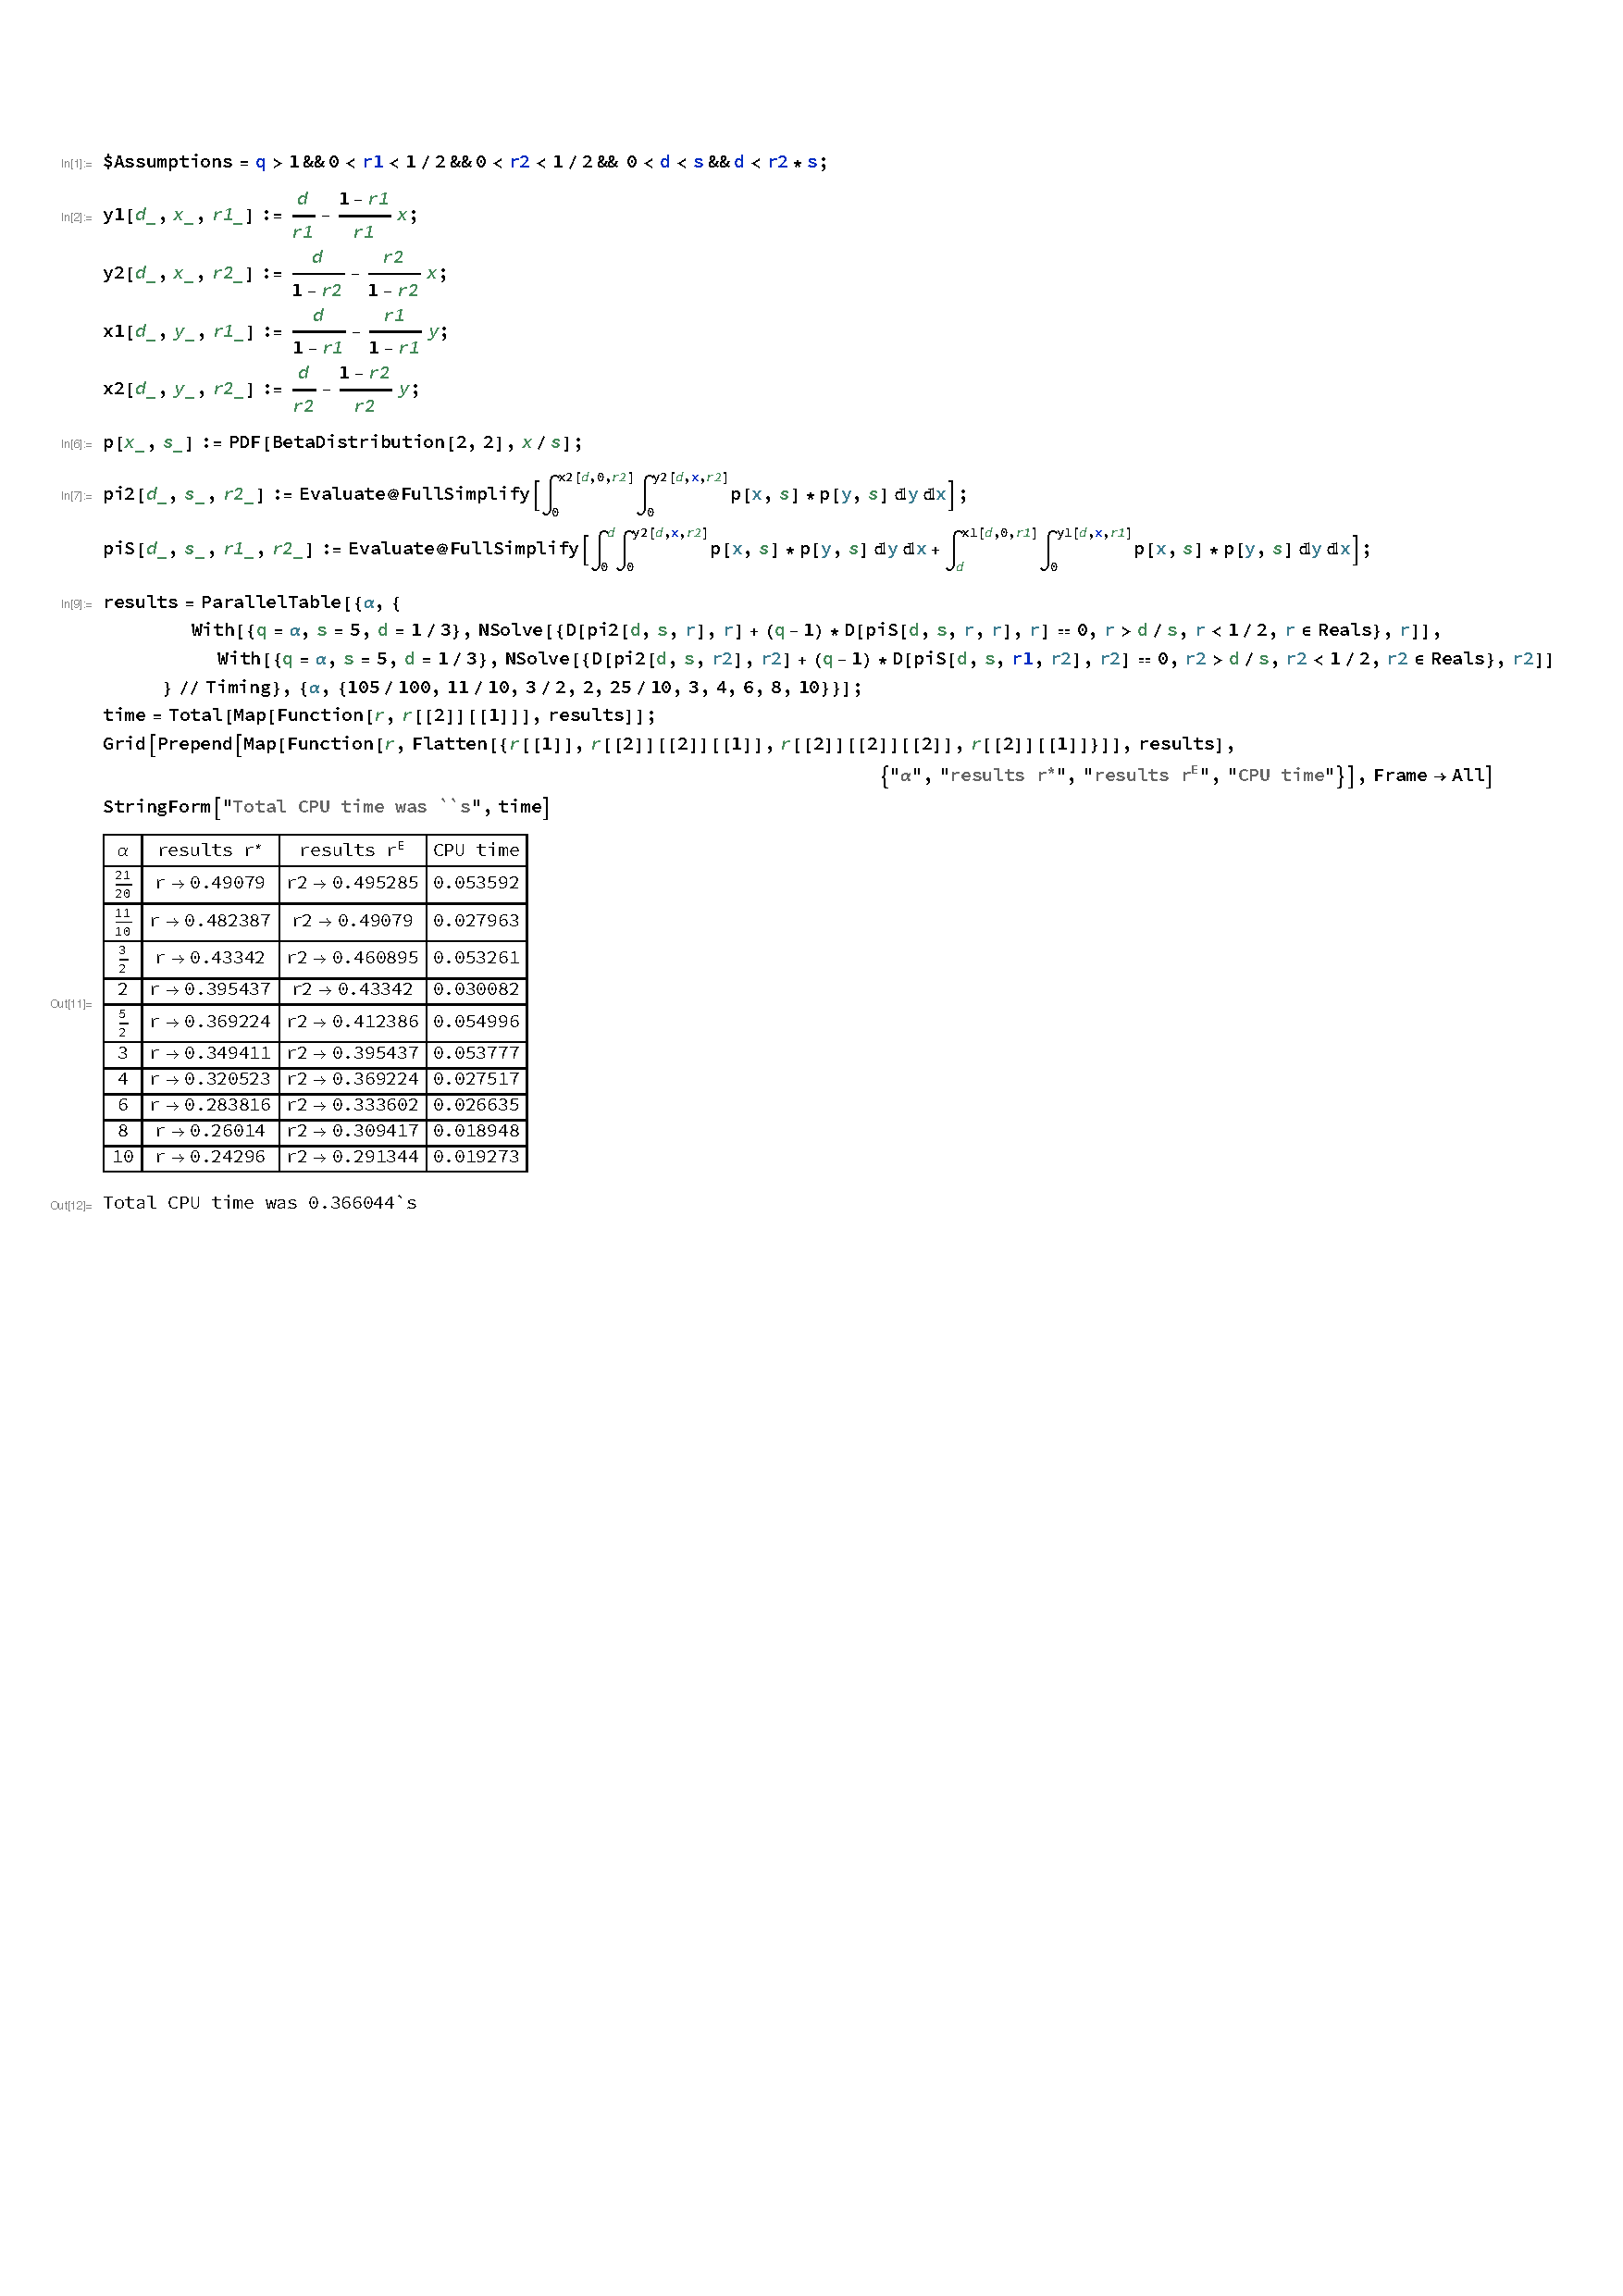
\includegraphics[scale=0.7]{figures/mathematica-source}
\end{sidewaystable}            \cleardoublepage{}

% References %%%%%%%%%%%%%%%%%%%%%%%%%%%%%%%%%%%%%%%%%%%%%%%%%%%%%%%%%%%%%%%%%%%
%%%%%%%%%%%%%%%%%%%%%%%%%%%%%%%%%%%%%%%%%%%%%%%%%%%%%%%%%%%%%%%%%%%%%%%%%%%%%%%%
\renewcommand{\chaptermark}[1]{\markboth{\thechapter\ #1}{}}
\renewcommand{\sectionmark}[1]{\markright{\thesection\ #1}}

\printbibliography[title=Literaturverzeichnis,heading=bibintoc] \cleardoublepage{}
\newpage\null\thispagestyle{empty}\newpage

\end{document}
